\chapter{Análise de Distribuição e Normalidade}
\label{chap:analise_distribuicao_normalidade}

Nesta seção, investigamos a forma das distribuições das métricas de conectividade, tanto nos seus valores “puros” quanto nas diferenças (median\_diff) entre condições (Pós – Pré). Inicialmente, apresentamos os histogramas das métricas originais extraídas dos sinais (PLI e CF-PLM), e em seguida, explicamos que para testar o efeito da estimulação, calculamos a diferença entre os valores pós e pré (por exemplo, pós‐sham menos pré‐sham). Finalmente, são apresentados os histogramas das diferenças e discutidas as implicações para a escolha dos testes estatísticos.

\section{Distribuição das Métricas de Conectividade (PLI e CF-PLM)}

\subsection{Distribuição dos Valores Puros}
Antes de subtrair os valores pré dos pós, as métricas de conectividade (PLI, PLV e CF-PLM) são extraídas diretamente dos sinais, refletindo as medidas originais sem a influência do efeito de estimulação. As figuras a seguir ilustram as distribuições “puras” dessas métricas para os diferentes grupos de canais (EEG-EEG e EEG-ECG) e faixas de frequência (delta, theta, alpha, beta e gamma).

\begin{figure}[htb]
    \centering
    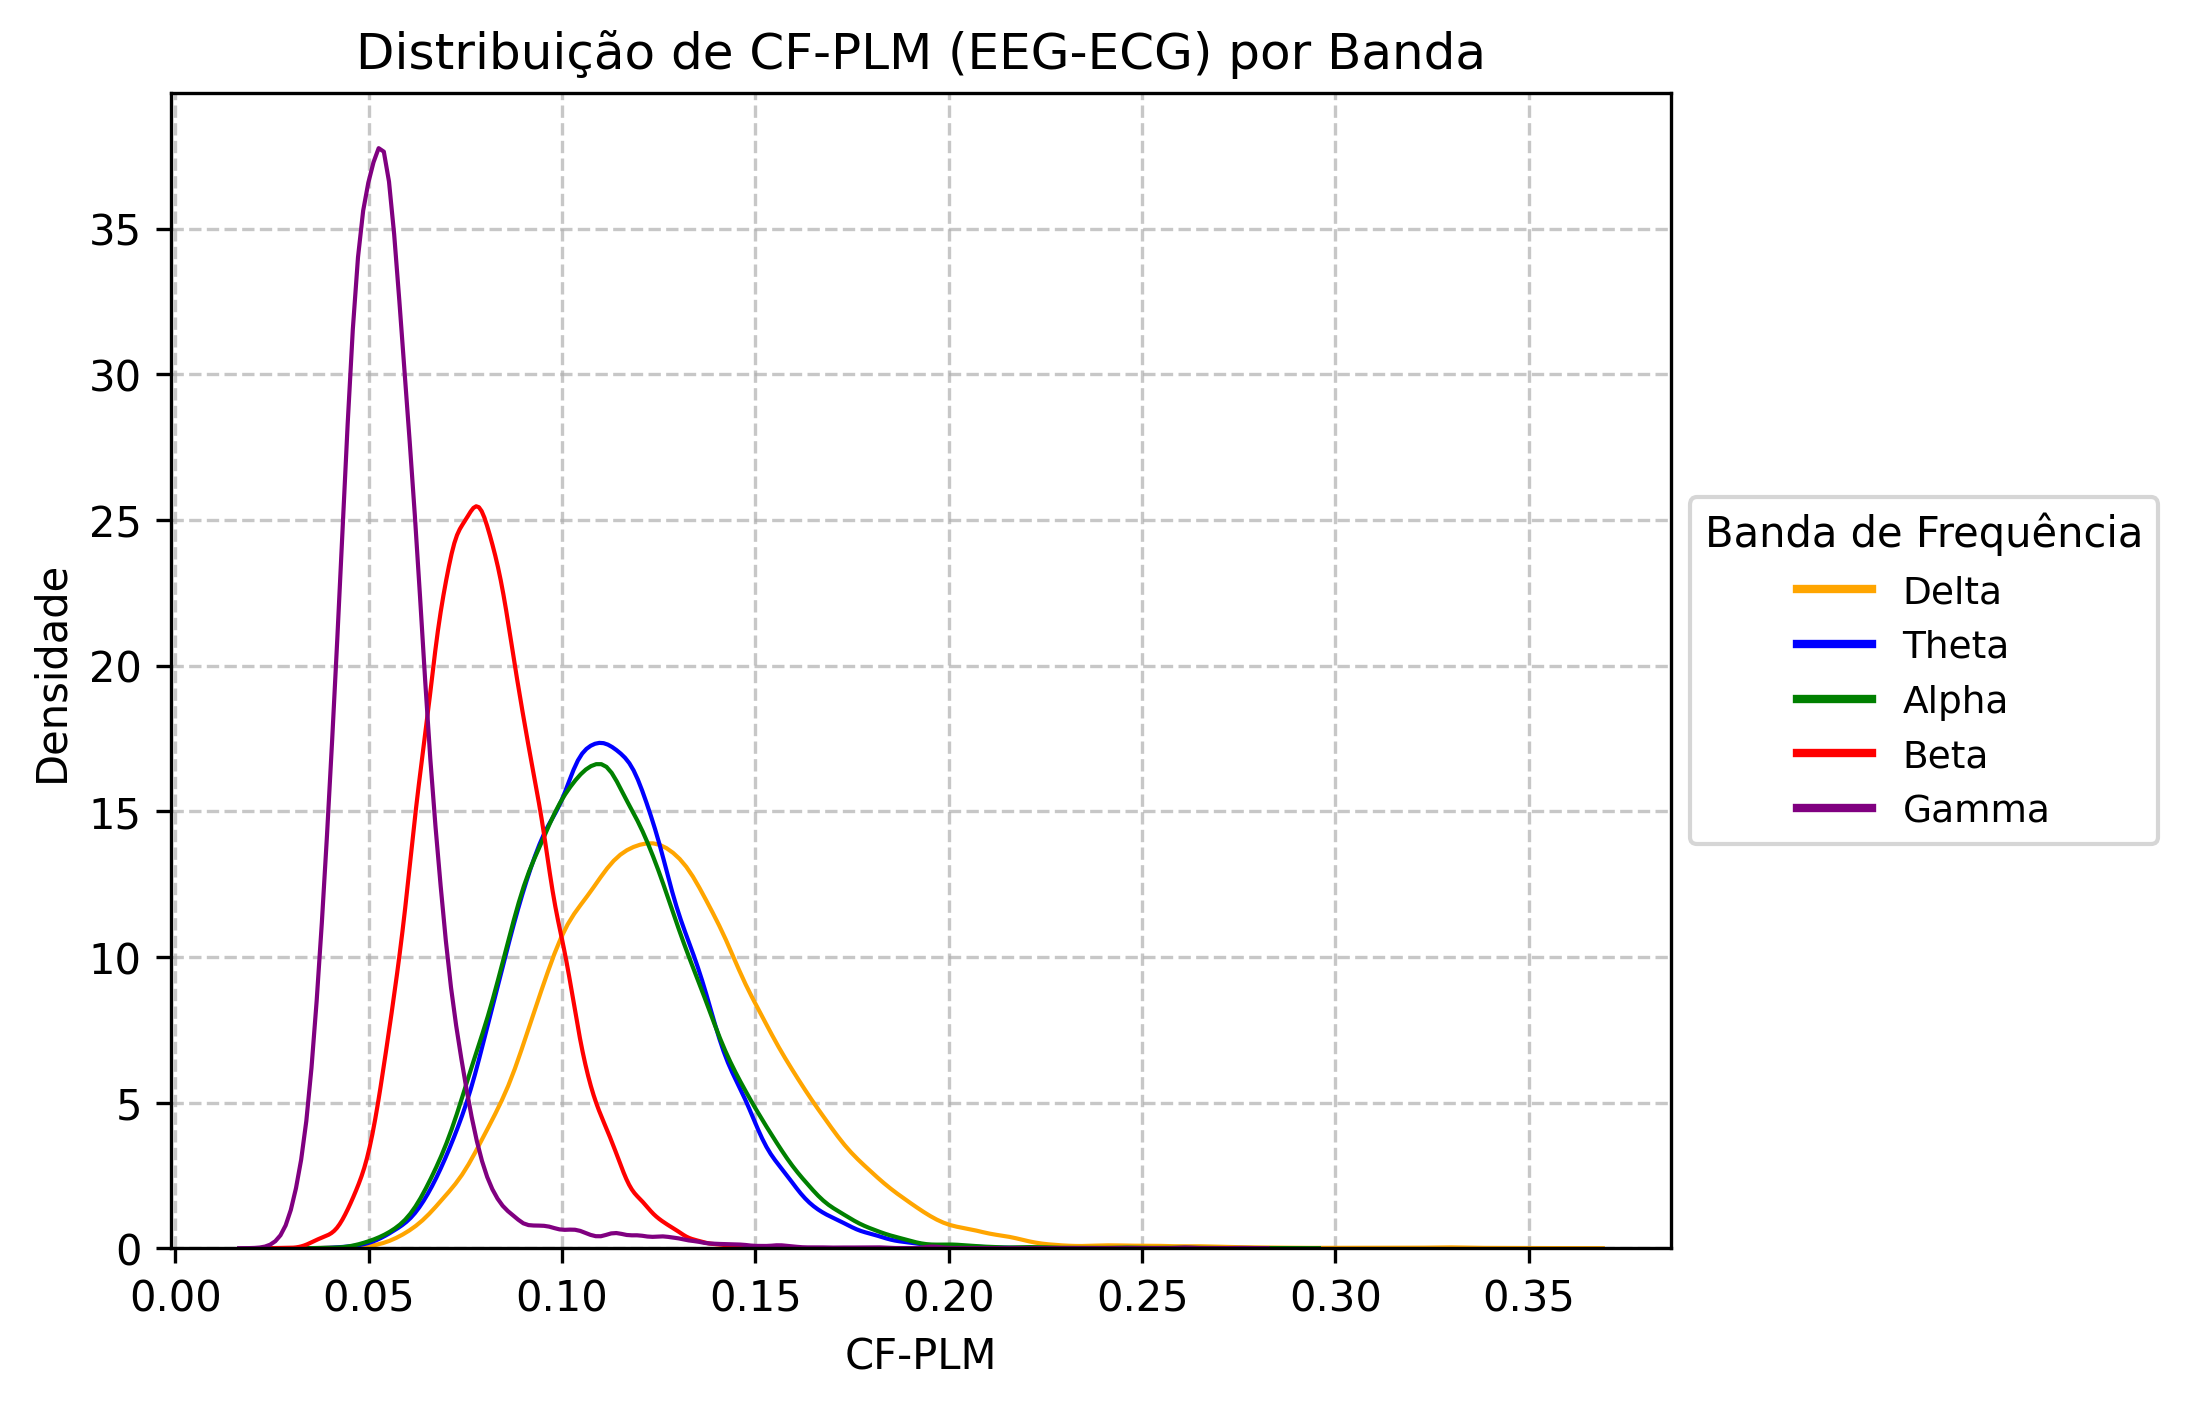
\includegraphics[width=0.7\textwidth]{figs/3_1_connectivity_metrics/Distribuição_de_CF-PLM_(EEG-ECG)_por_Banda.png}
    \caption{Distribuição de CF-PLM (EEG-ECG) por banda. Observa-se a concentração dos valores em torno de faixas mais baixas (próximas de 0), com maior densidade para a banda delta (linha vermelha) e theta (linha azul).}
    \label{fig:cfplm_eeg_ecg}
\end{figure}

\begin{figure}[htb]
    \centering
    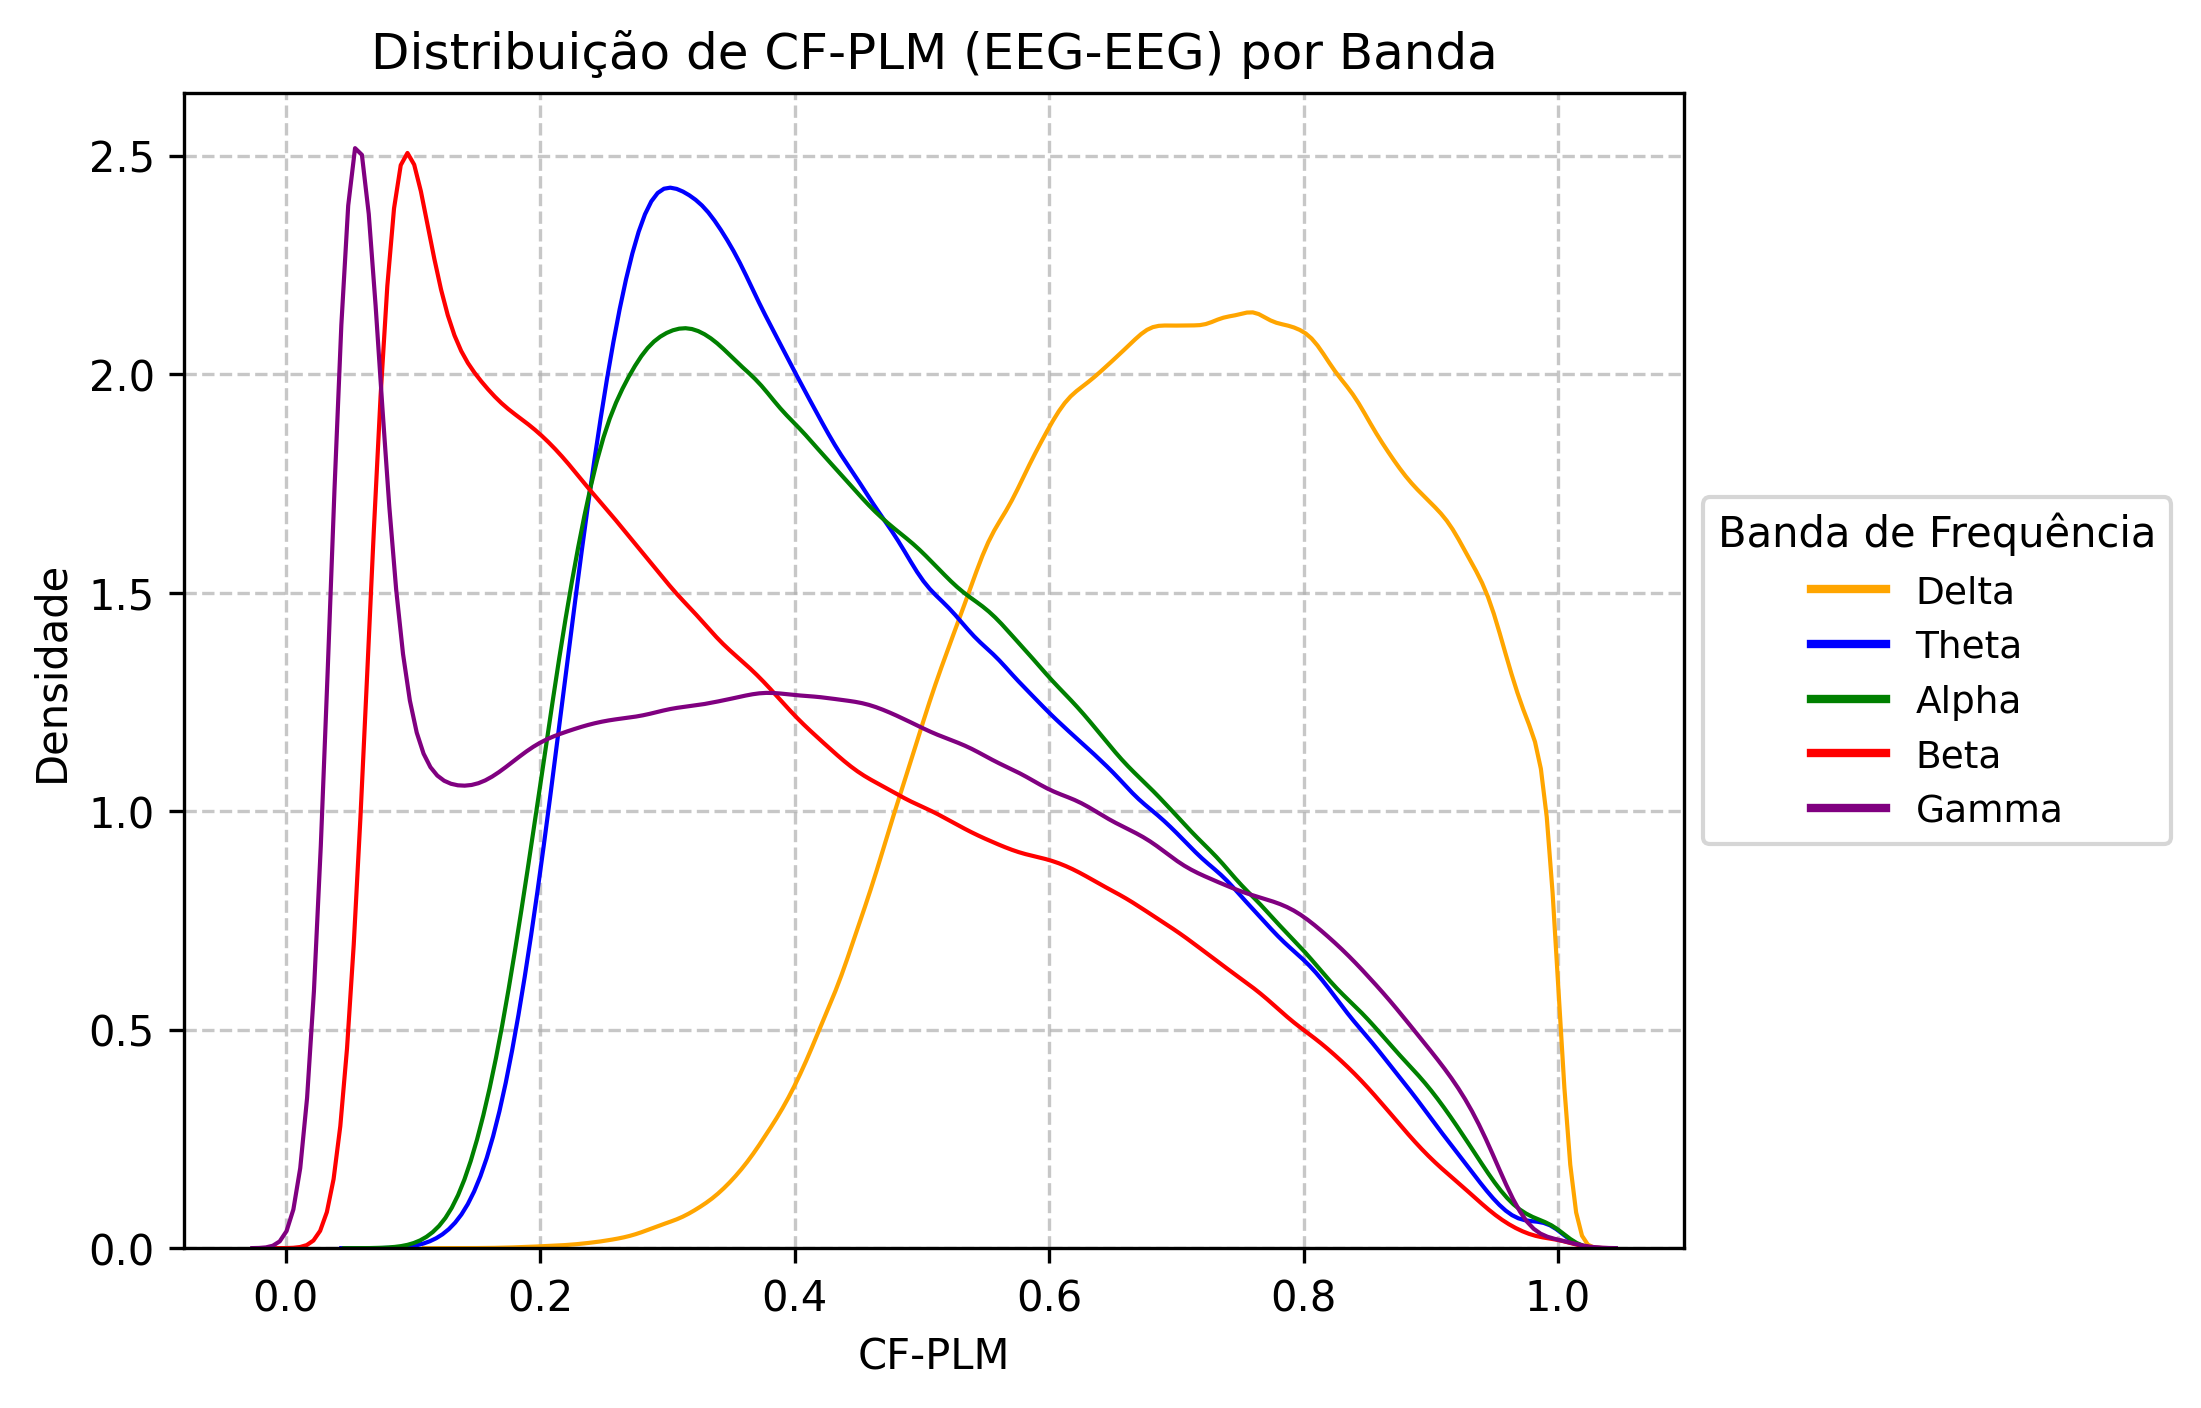
\includegraphics[width=0.7\textwidth]{figs/3_1_connectivity_metrics/Distribuição_de_CF-PLM_(EEG-EEG)_por_Banda.png}
    \caption{Distribuição de CF-PLM (EEG-EEG) por banda. Nesse caso, alguns pares apresentam valores mais elevados, evidenciando maior acoplamento \emph{cross-frequency} dentro do EEG, especialmente em alpha e gamma.}
    \label{fig:cfplm_eeg_eeg}
\end{figure}

\begin{figure}[htb]
    \centering
    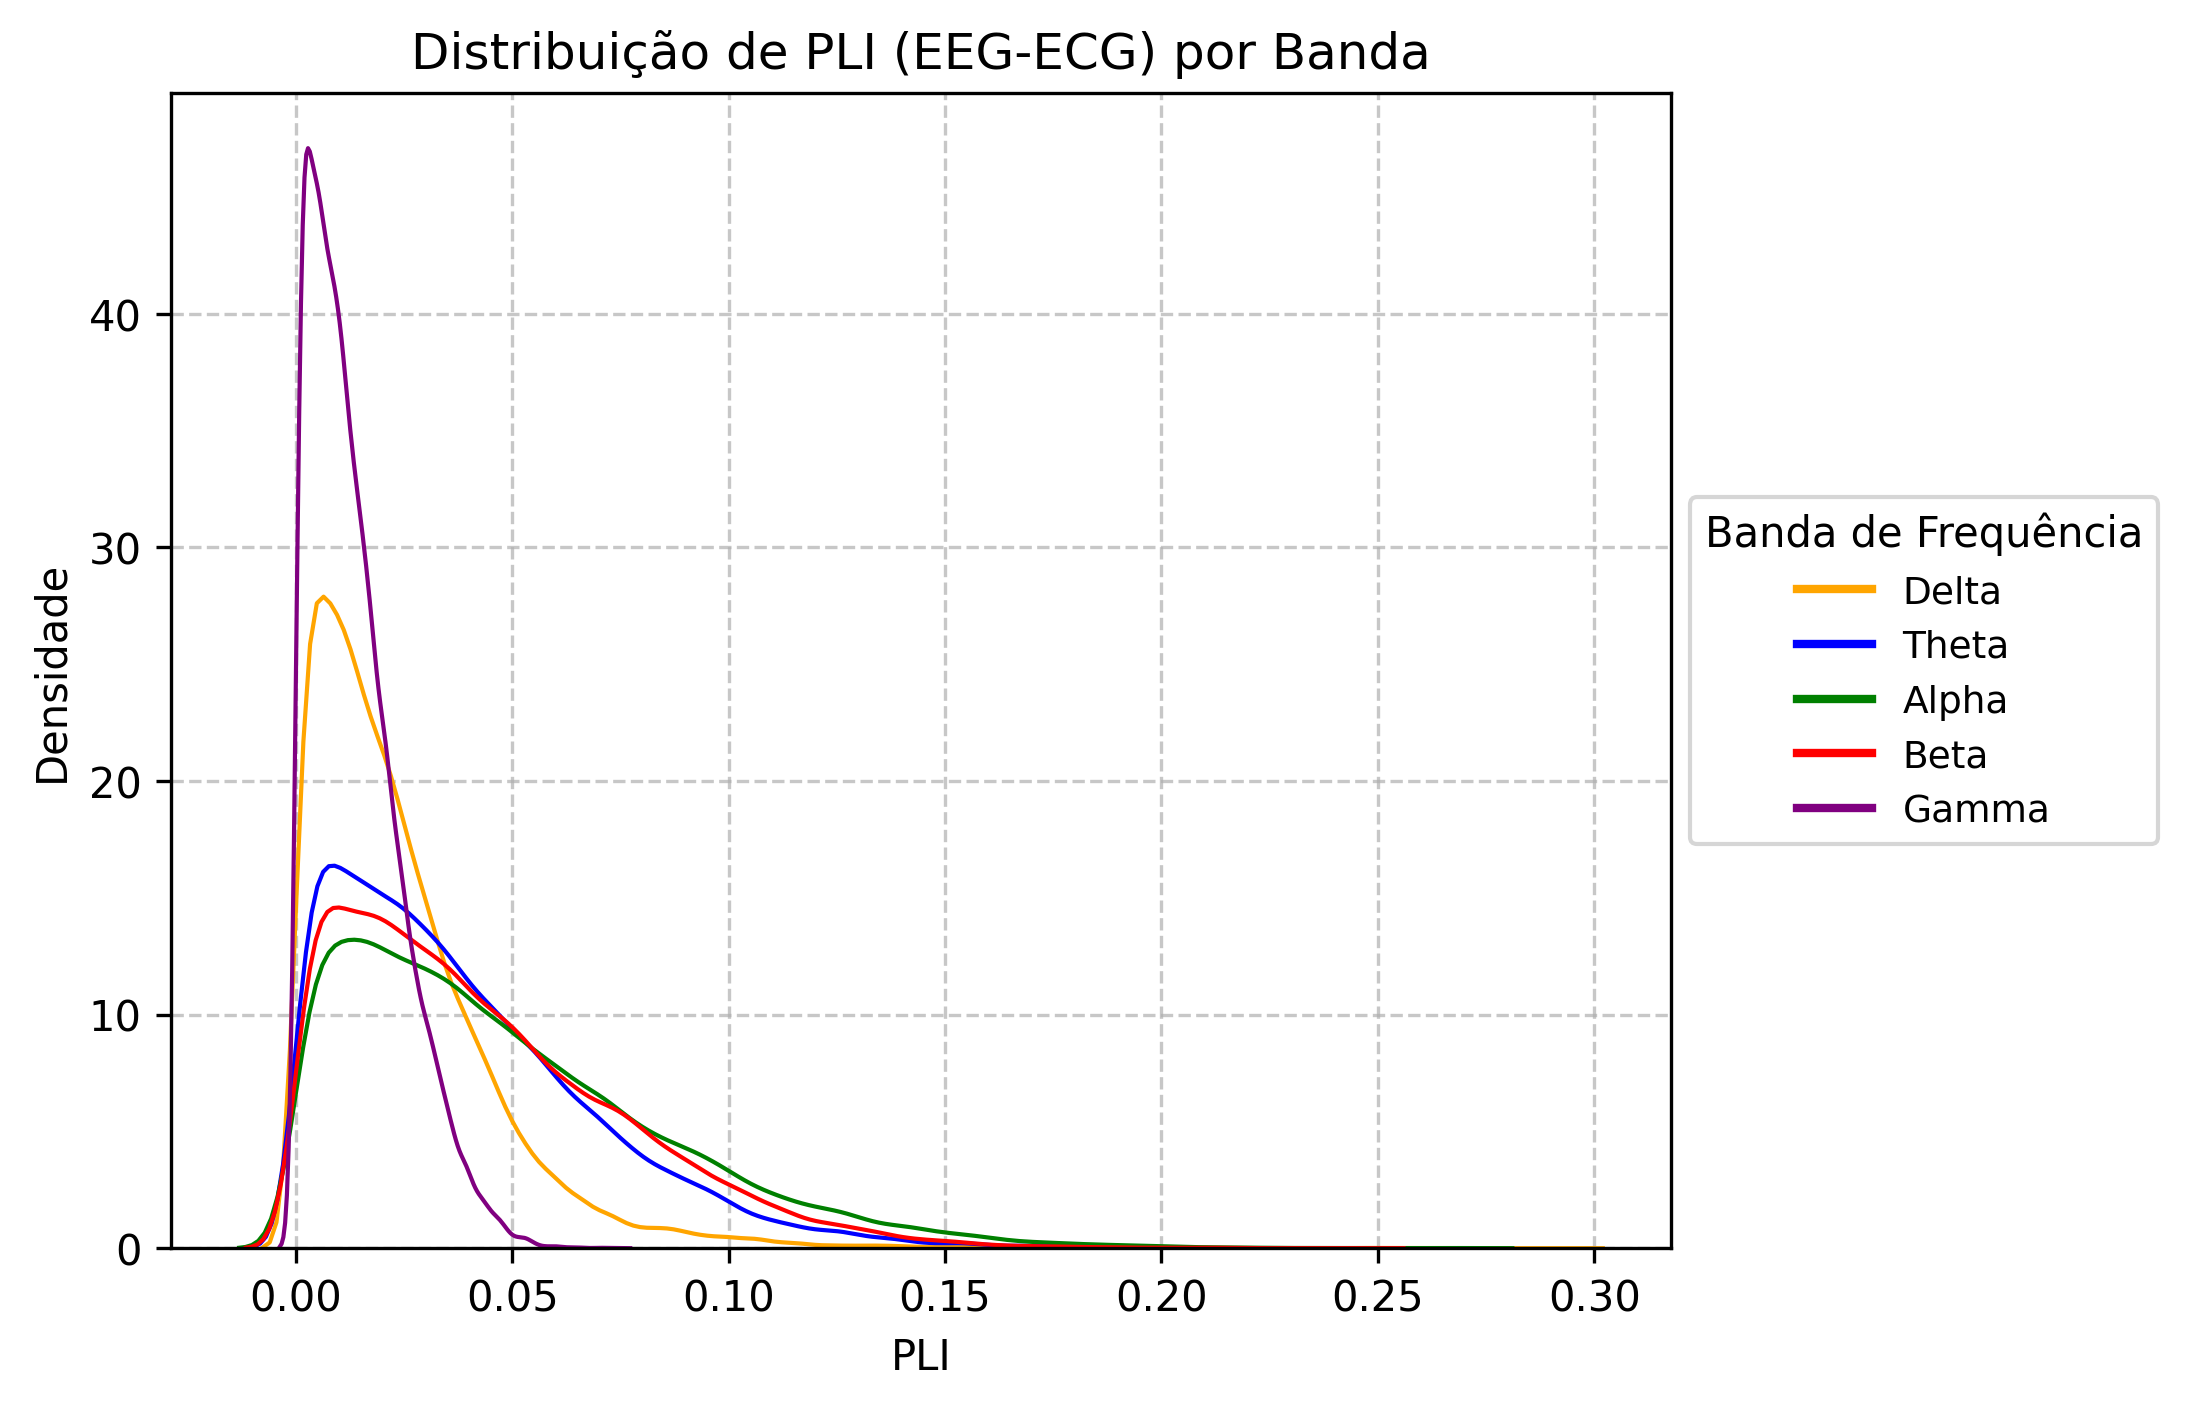
\includegraphics[width=0.7\textwidth]{figs/3_1_connectivity_metrics/Distribuição_de_PLI_(EEG-ECG)_por_Banda.png}
    \caption{Distribuição de PLI (EEG-ECG) por banda. Os valores tendem a se concentrar muito próximos de zero, sugerindo que a maioria dos pares EEG-ECG não apresenta \emph{phase lag} robusto em bandas iso-frequenciais.}
    \label{fig:pli_eeg_ecg}
\end{figure}

\begin{figure}[htb]
    \centering
    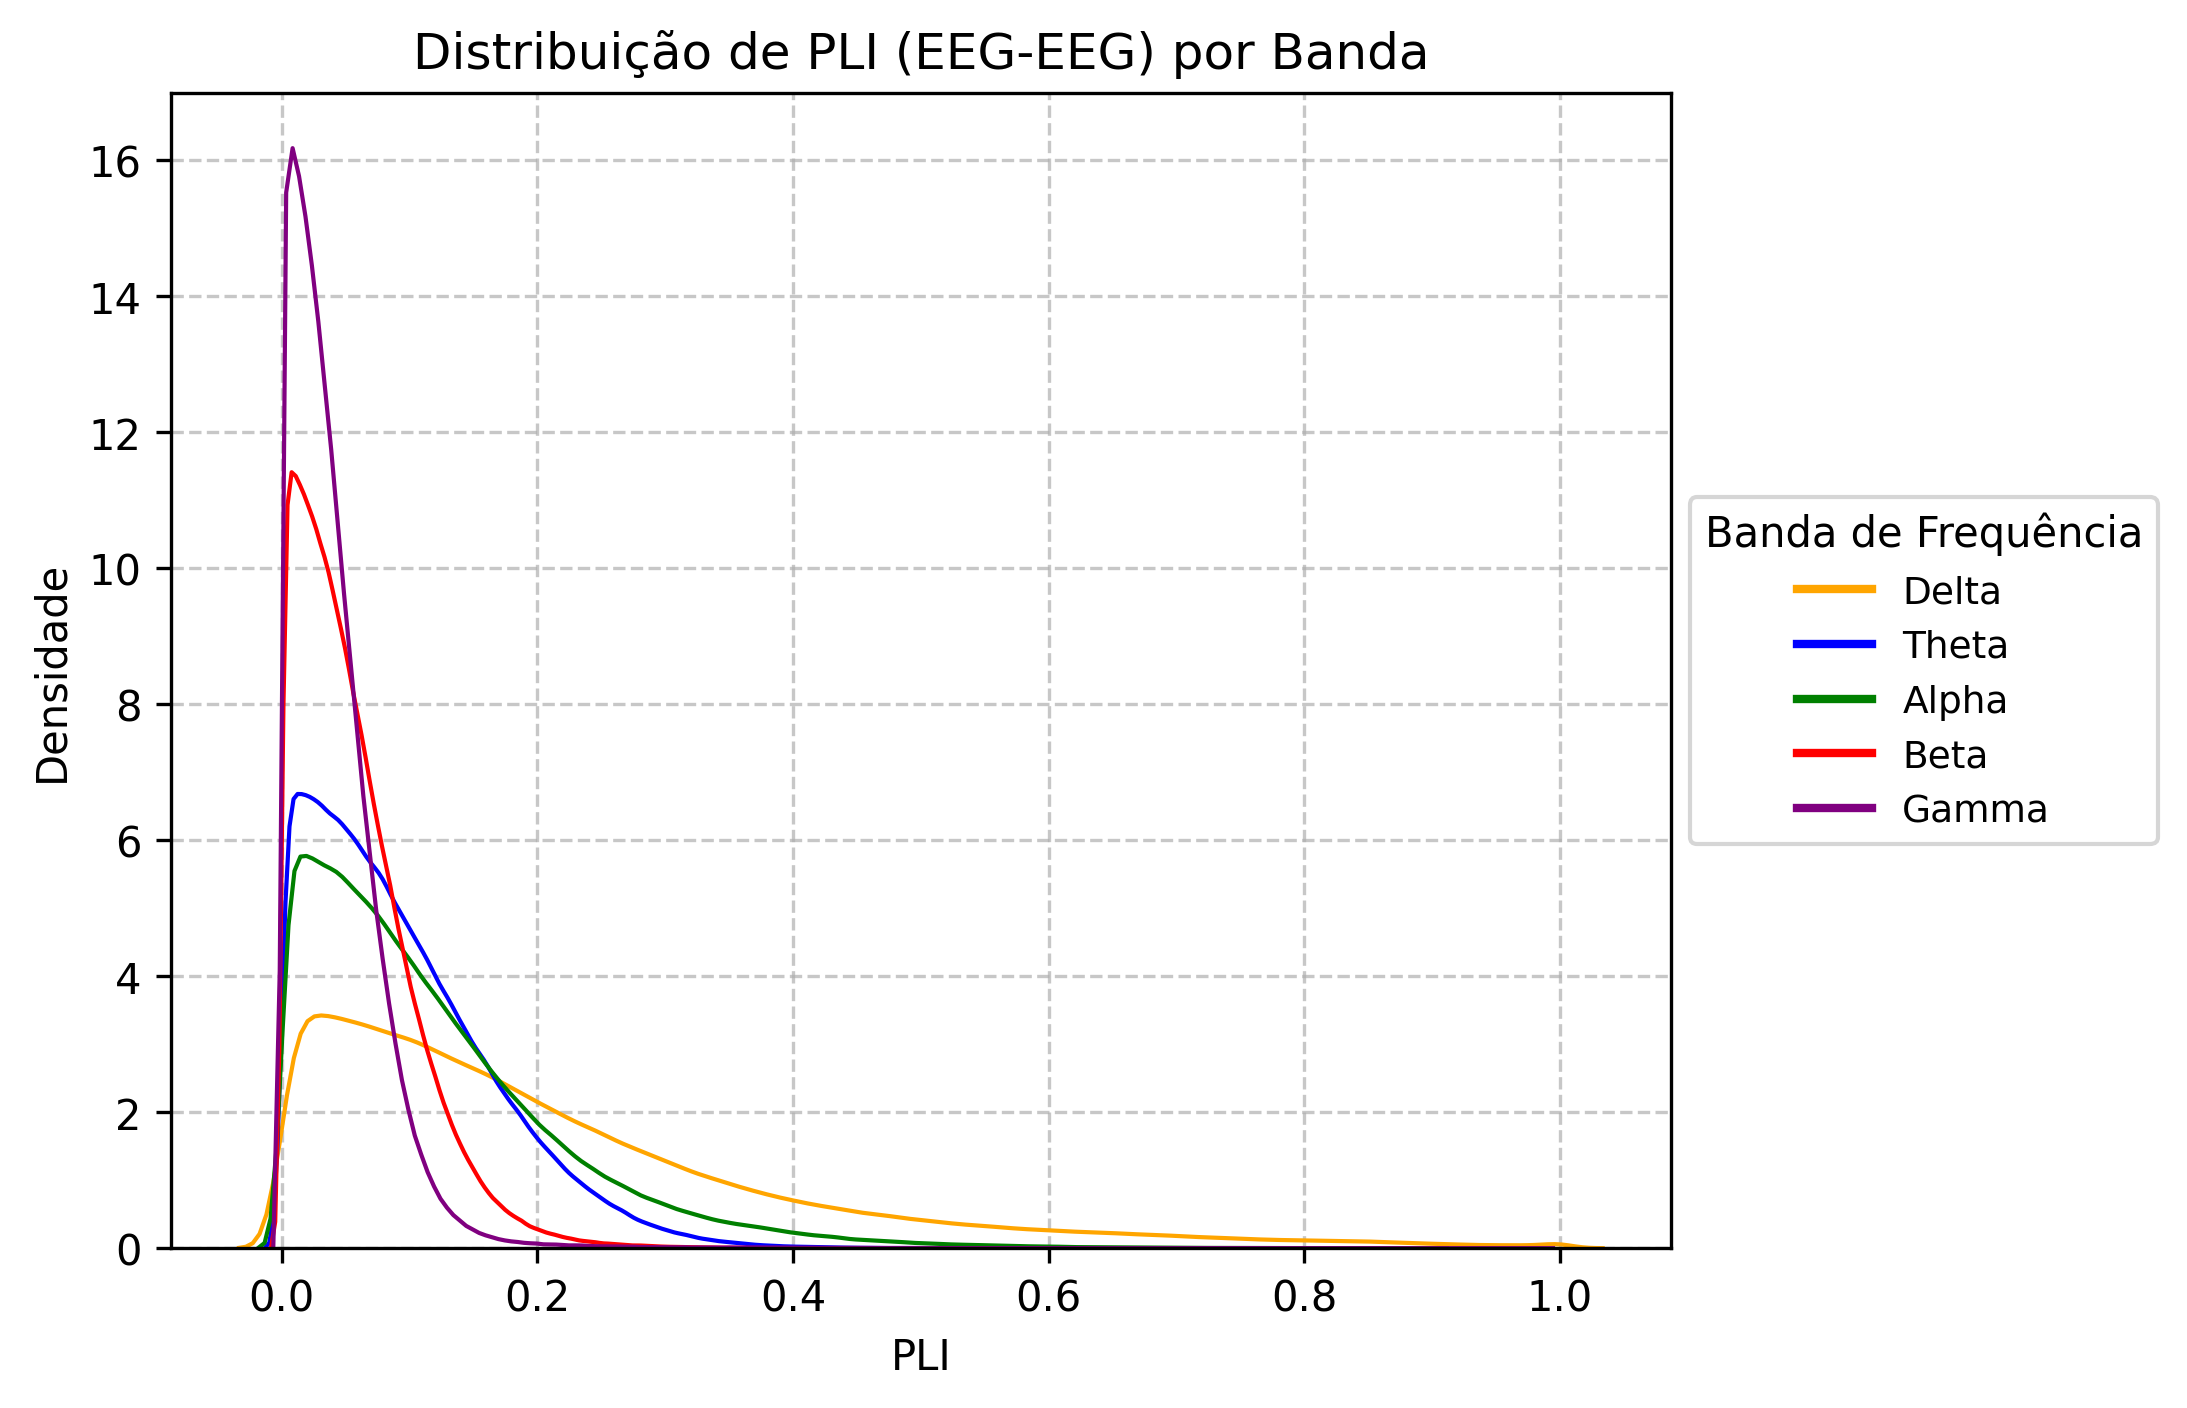
\includegraphics[width=0.7\textwidth]{figs/3_1_connectivity_metrics/Distribuição_de_PLI_(EEG-EEG)_por_Banda.png}
    \caption{Distribuição de PLI (EEG-EEG) por banda. Embora a maior parte dos valores se concentre em torno de zero, algumas bandas (como alpha e gamma) apresentam caudas mais extensas, indicando pares de canais com defasagem de fase mais consistente.}
    \label{fig:pli_eeg_eeg}
\end{figure}

\begin{figure}[htb]
    \centering
    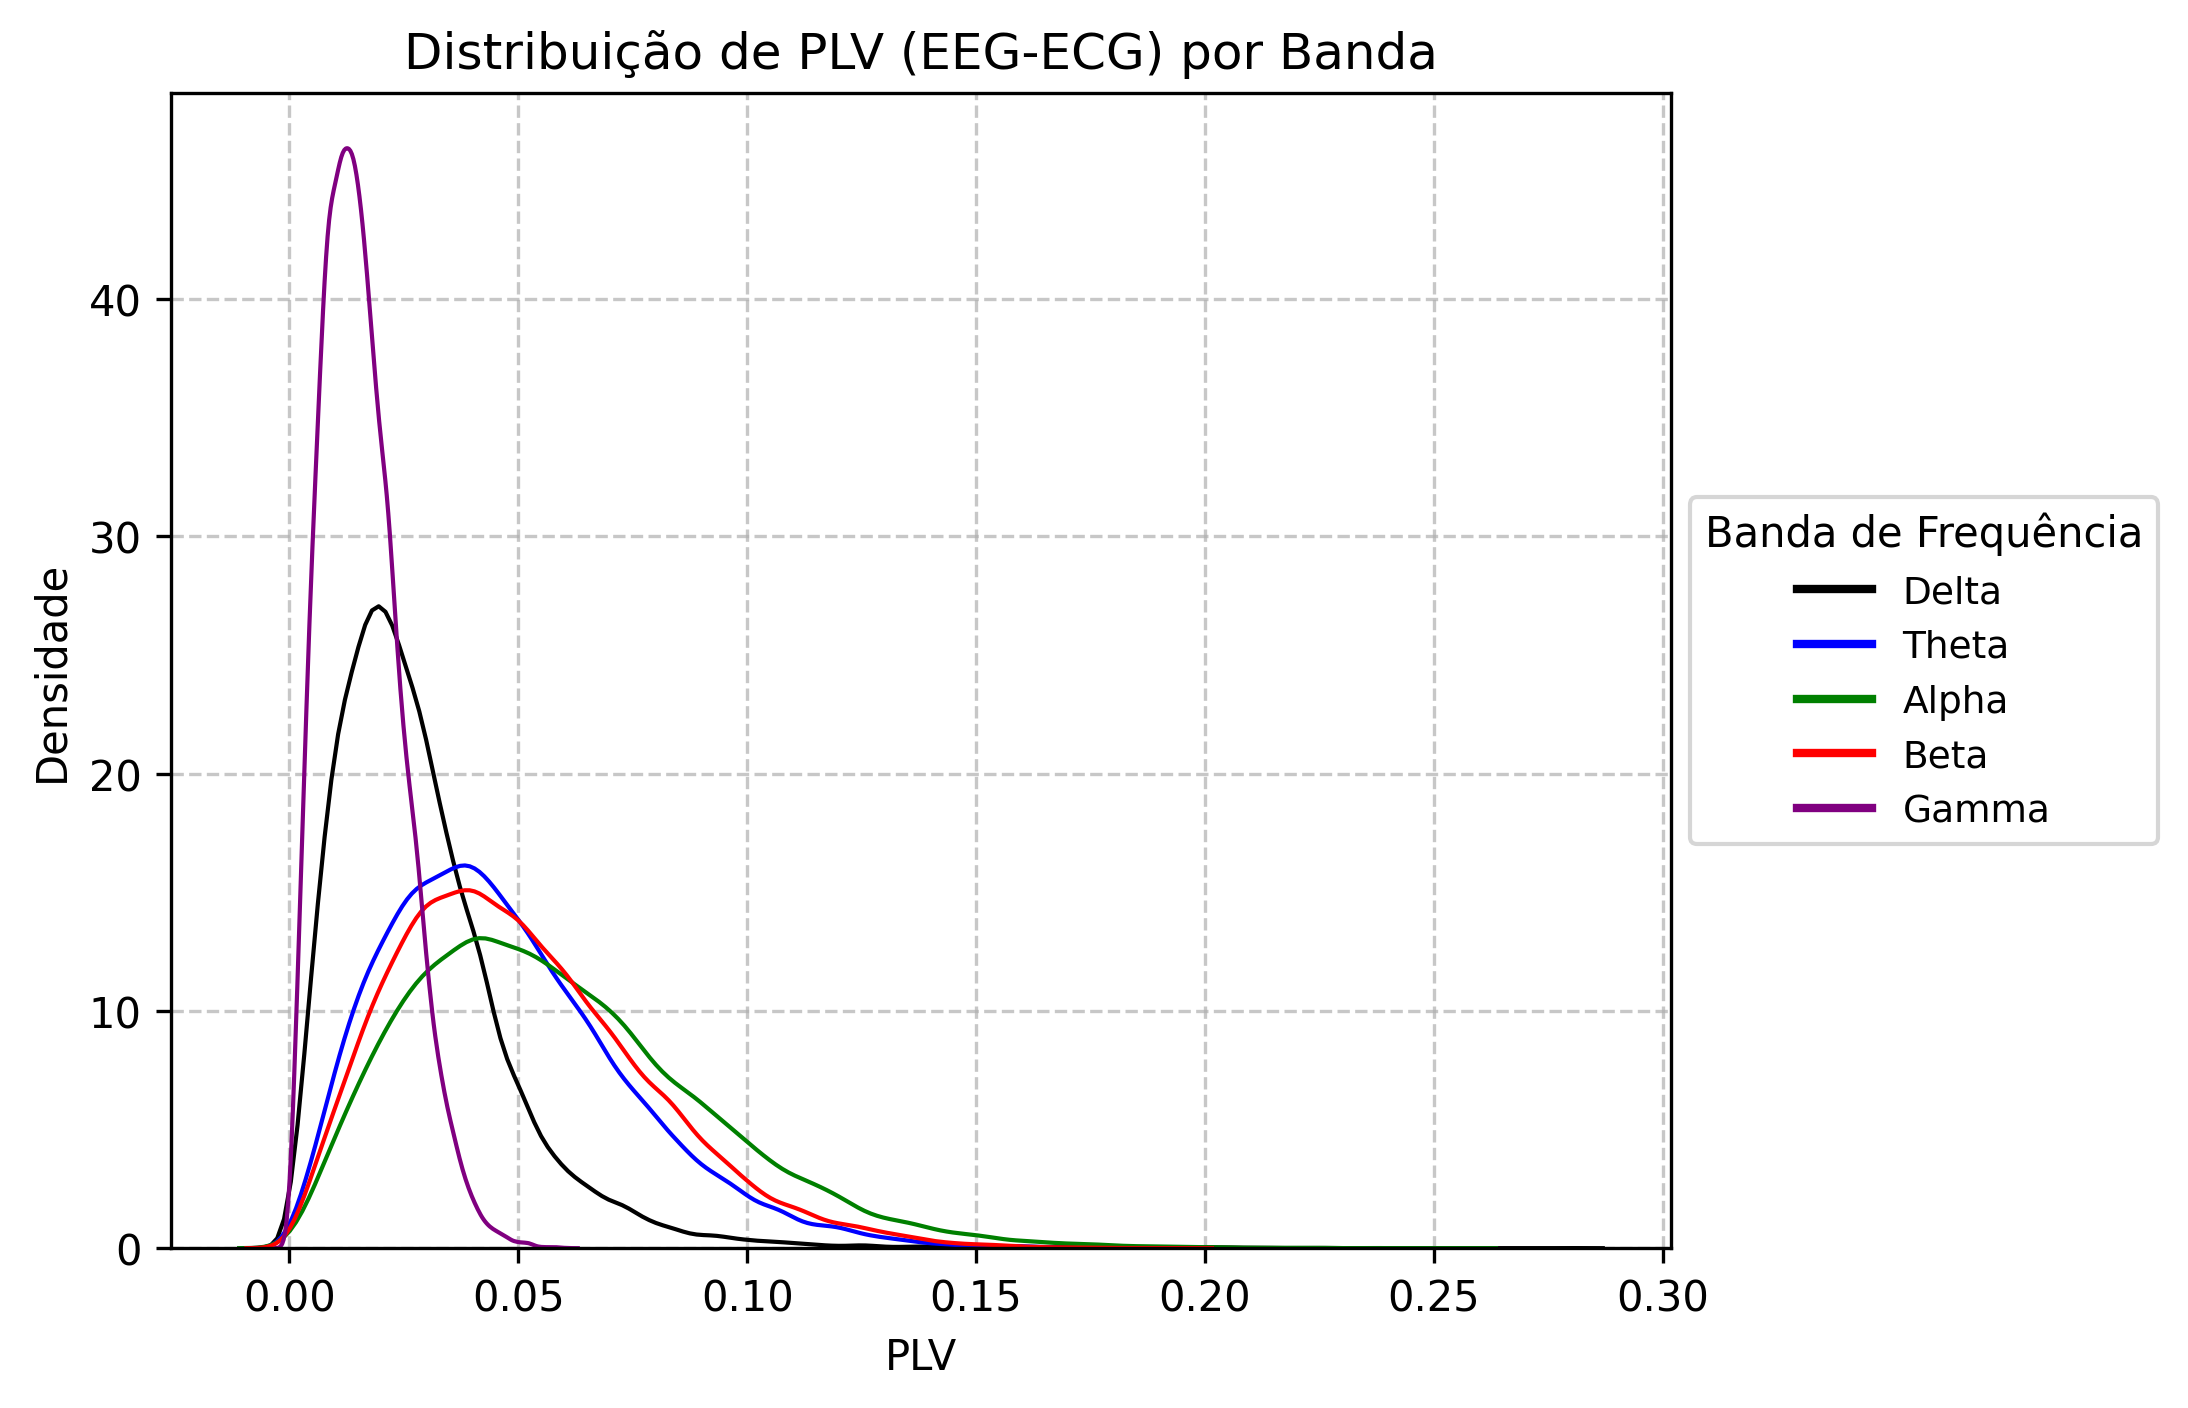
\includegraphics[width=0.7\textwidth]{figs/3_1_connectivity_metrics/Distribuição_de_PLV_(EEG-ECG)_por_Banda.png}
    \caption{Distribuição de PLV (EEG-ECG) por banda. Nota-se grande aglomeração de valores próximos de zero, revelando baixa coerência de fase iso-frequencial entre o sinal cardíaco e as oscilações cerebrais na maioria dos pares.}
    \label{fig:plv_eeg_ecg}
\end{figure}

\begin{figure}[htb]
    \centering
    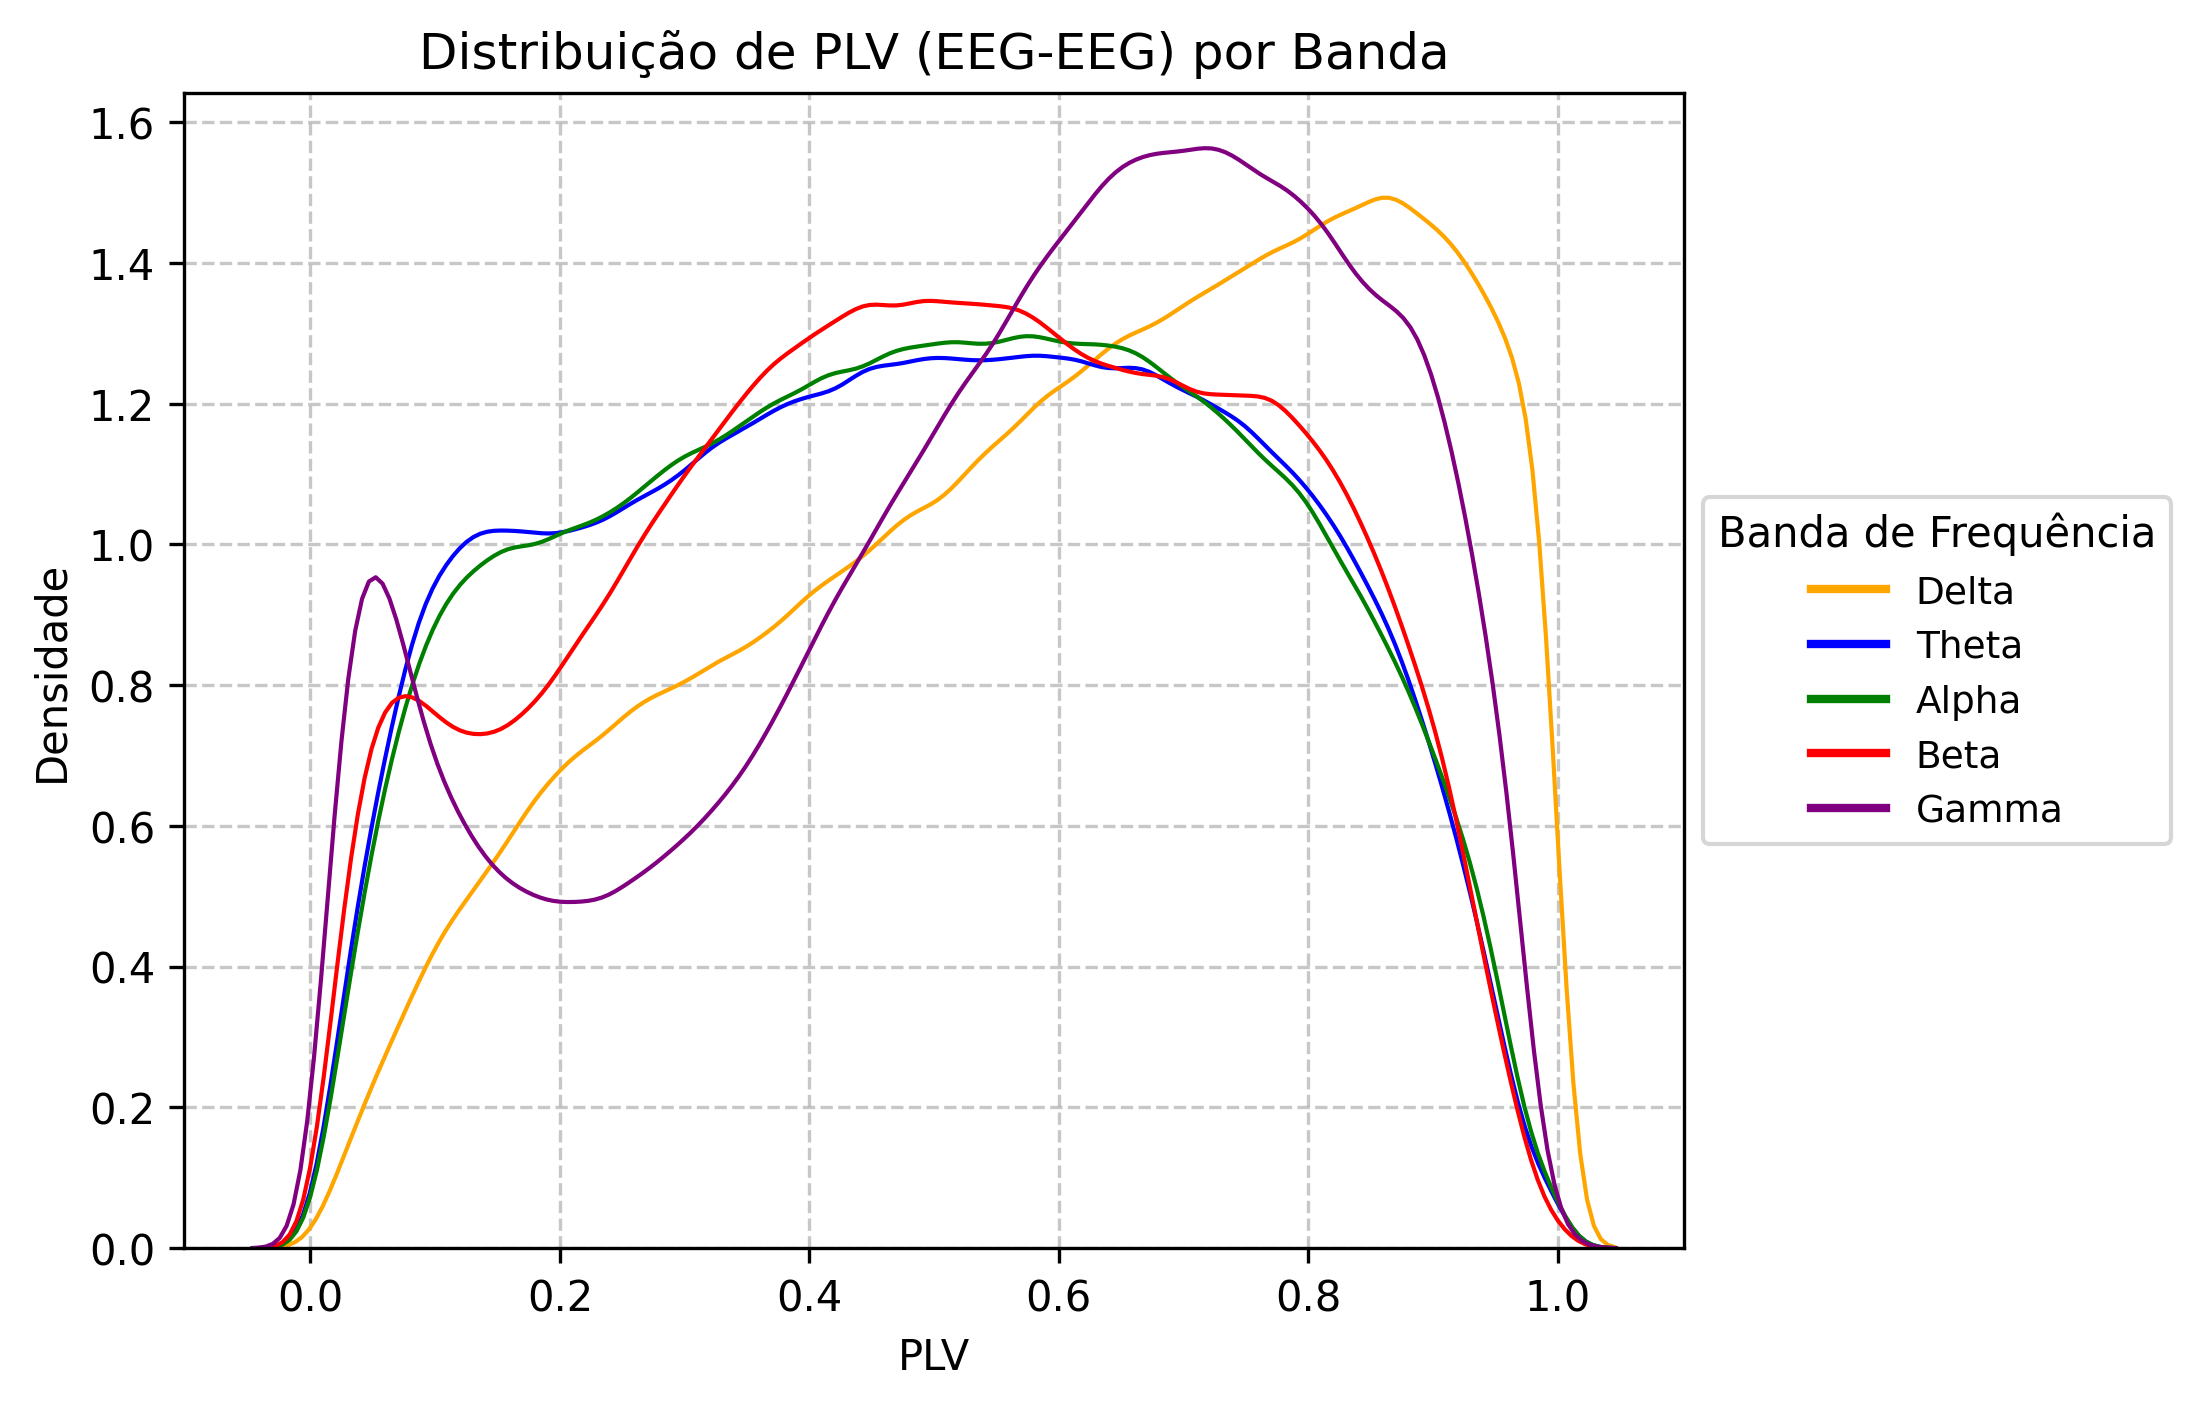
\includegraphics[width=0.7\textwidth]{figs/3_1_connectivity_metrics/Distribuição_de_PLV_(EEG-EEG)_por_Banda.png}
    \caption{Distribuição de PLV (EEG-EEG) por banda. Alguns valores atingem níveis elevados (acima de 0.5), indicando que certos pares de canais EEG podem apresentar forte \emph{phase locking} em determinadas faixas de frequência, especialmente em gamma.}
    \label{fig:plv_eeg_eeg}
\end{figure}

No geral, observa-se que:
\begin{itemize}
    \item \textbf{EEG-ECG}: As métricas PLI e PLV concentram-se em valores muito baixos, indicando fraca sincronização de fase iso-frequencial entre o ritmo cardíaco e o sinal cerebral. Em contrapartida, o CF-PLM apresenta valores um pouco maiores, apontando para um acoplamento \emph{cross-frequency} pontual.
    \item \textbf{EEG-EEG}: Tanto PLI quanto PLV exibem distribuições que podem se estender para valores mais altos, sugerindo a presença de sincronizações mais robustas entre canais cerebrais na mesma banda. O CF-PLM, por sua vez, chega a atingir níveis ainda maiores, evidenciando interações entre faixas de frequência distintas (p.\,ex.\ oscilações lentas e rápidas).
\end{itemize}

Essas observações fornecem uma visão inicial sobre o comportamento das métricas “puras” de conectividade, servindo de ponto de partida para as comparações entre condições (Pós e Pré) apresentadas na próxima subseção.

\subsection{Distribuição das Diferenças (Median Diff)}
Para testar o efeito da estimulação (\emph{cathodic} versus \emph{sham}), os valores medidos após a intervenção (pós) foram comparados com os valores obtidos antes da intervenção (pré). Assim, a métrica de diferença (\texttt{median\_diff}) é calculada subtraindo-se o valor pré do valor pós (por exemplo, pós-sham $-$ pré-sham). Essa operação visa isolar o efeito da intervenção, eliminando variações comuns que possam estar presentes independentemente da estimulação.

As distribuições das diferenças foram, então, avaliadas por meio de histogramas com \emph{Kernel Density Estimation} (KDE) para as métricas de PLI e CF-PLM, conforme ilustrado nas figuras abaixo:

\begin{figure}[htb]
    \centering
    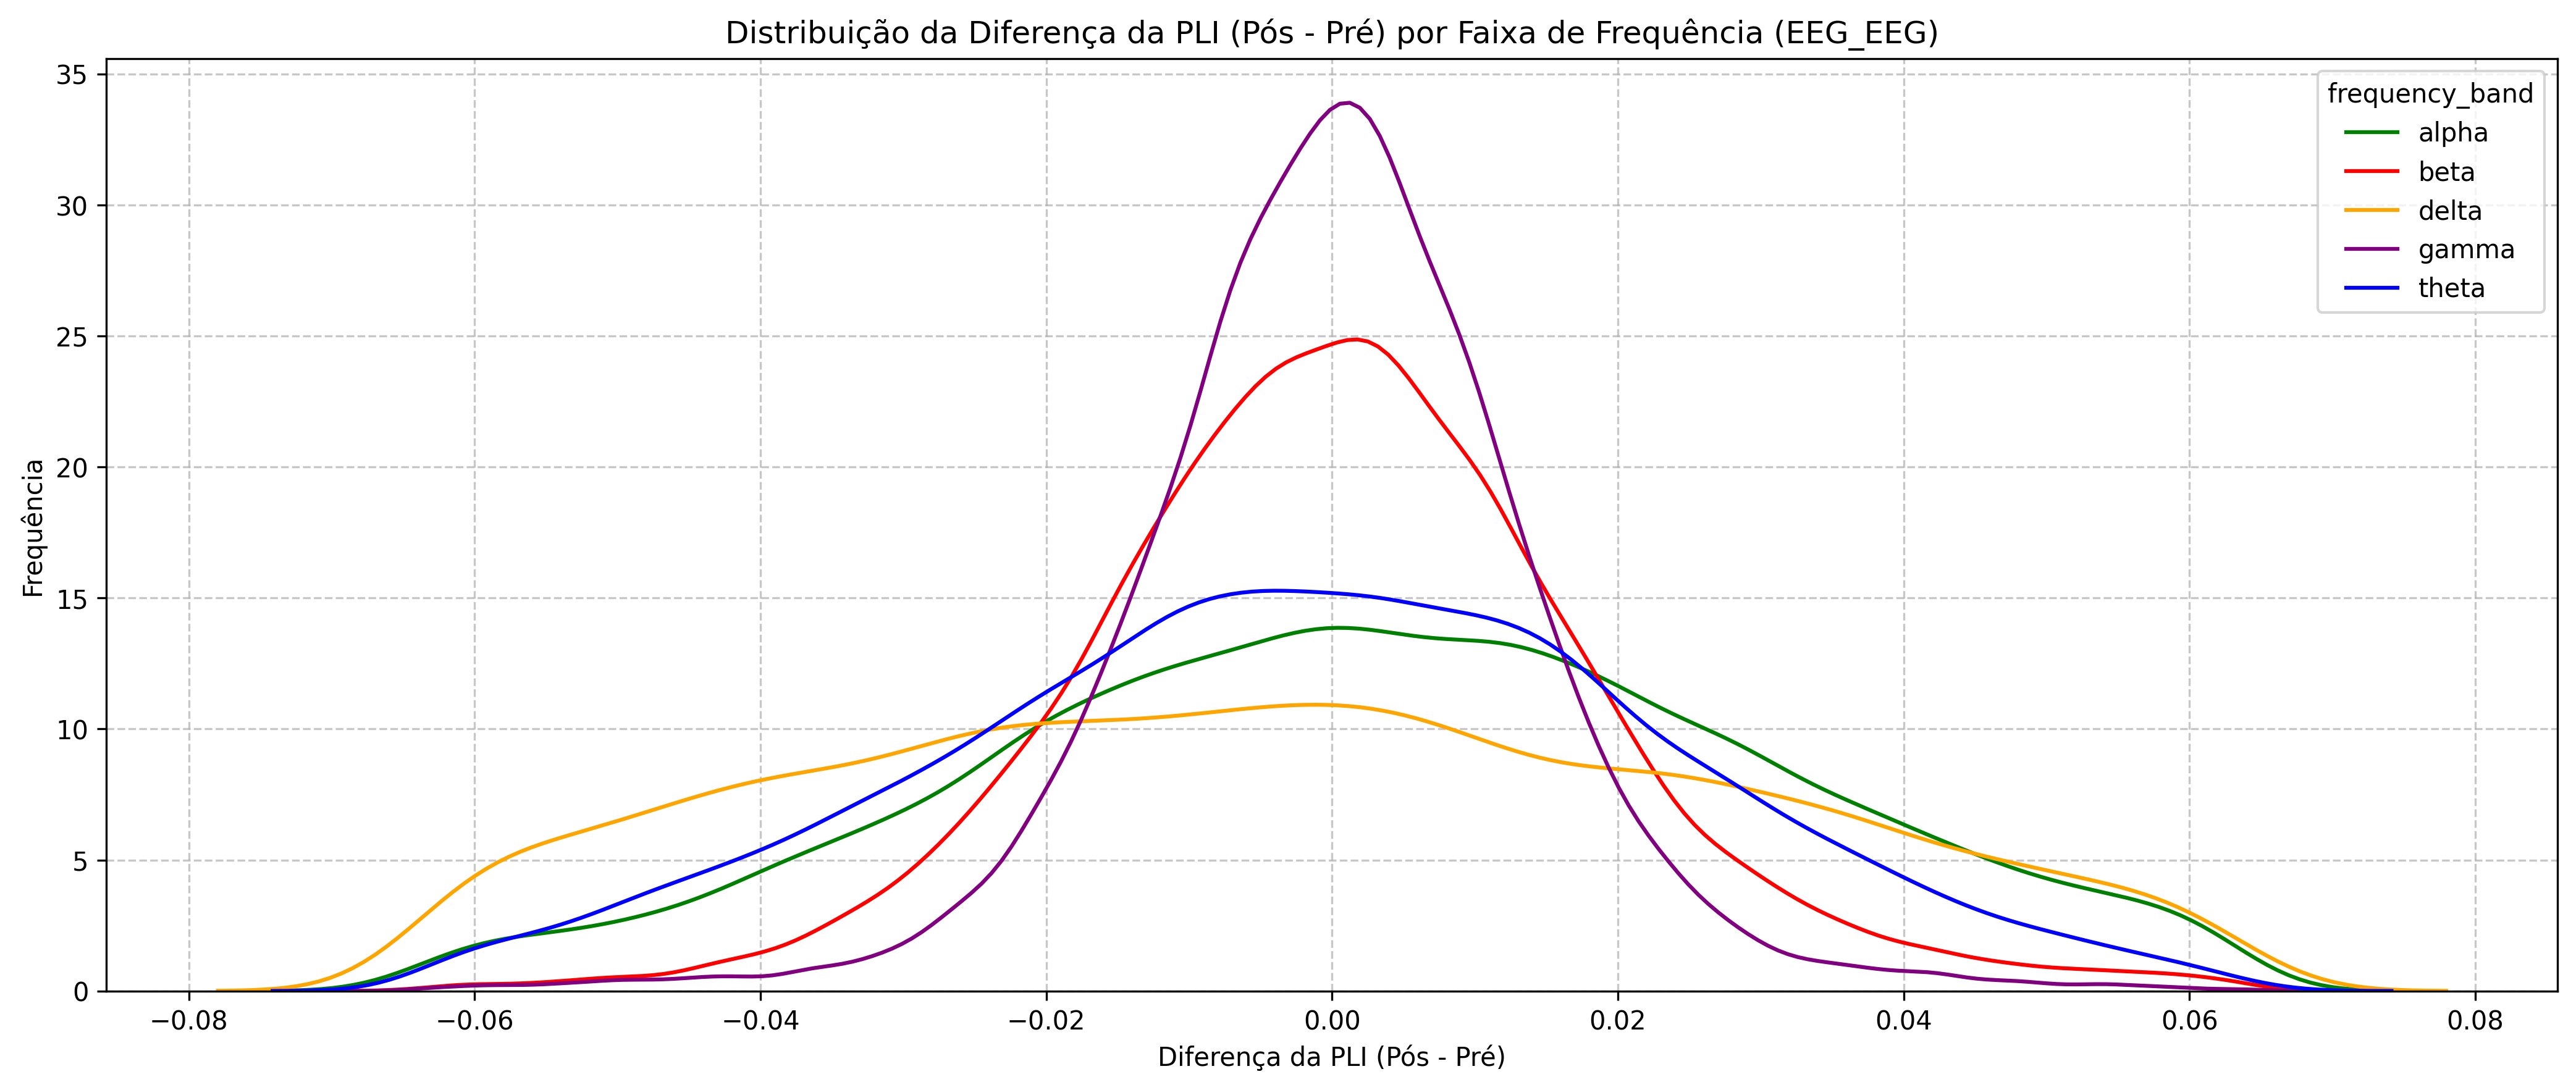
\includegraphics[width=0.8\textwidth]{figs/6_distribuicao_metricas_conectividade/Distribuição_da_Diferença_da_PLI_(Pós_-_Pré)_por_Faixa_de_Frequência_EEG_EEG.png}
    \caption{Distribuição da diferença da PLI (Pós -- Pré) por faixa de frequência para EEG-EEG.}
    \label{fig:pli_freq_eeg_eeg}
\end{figure}

\begin{figure}[htb]
    \centering
    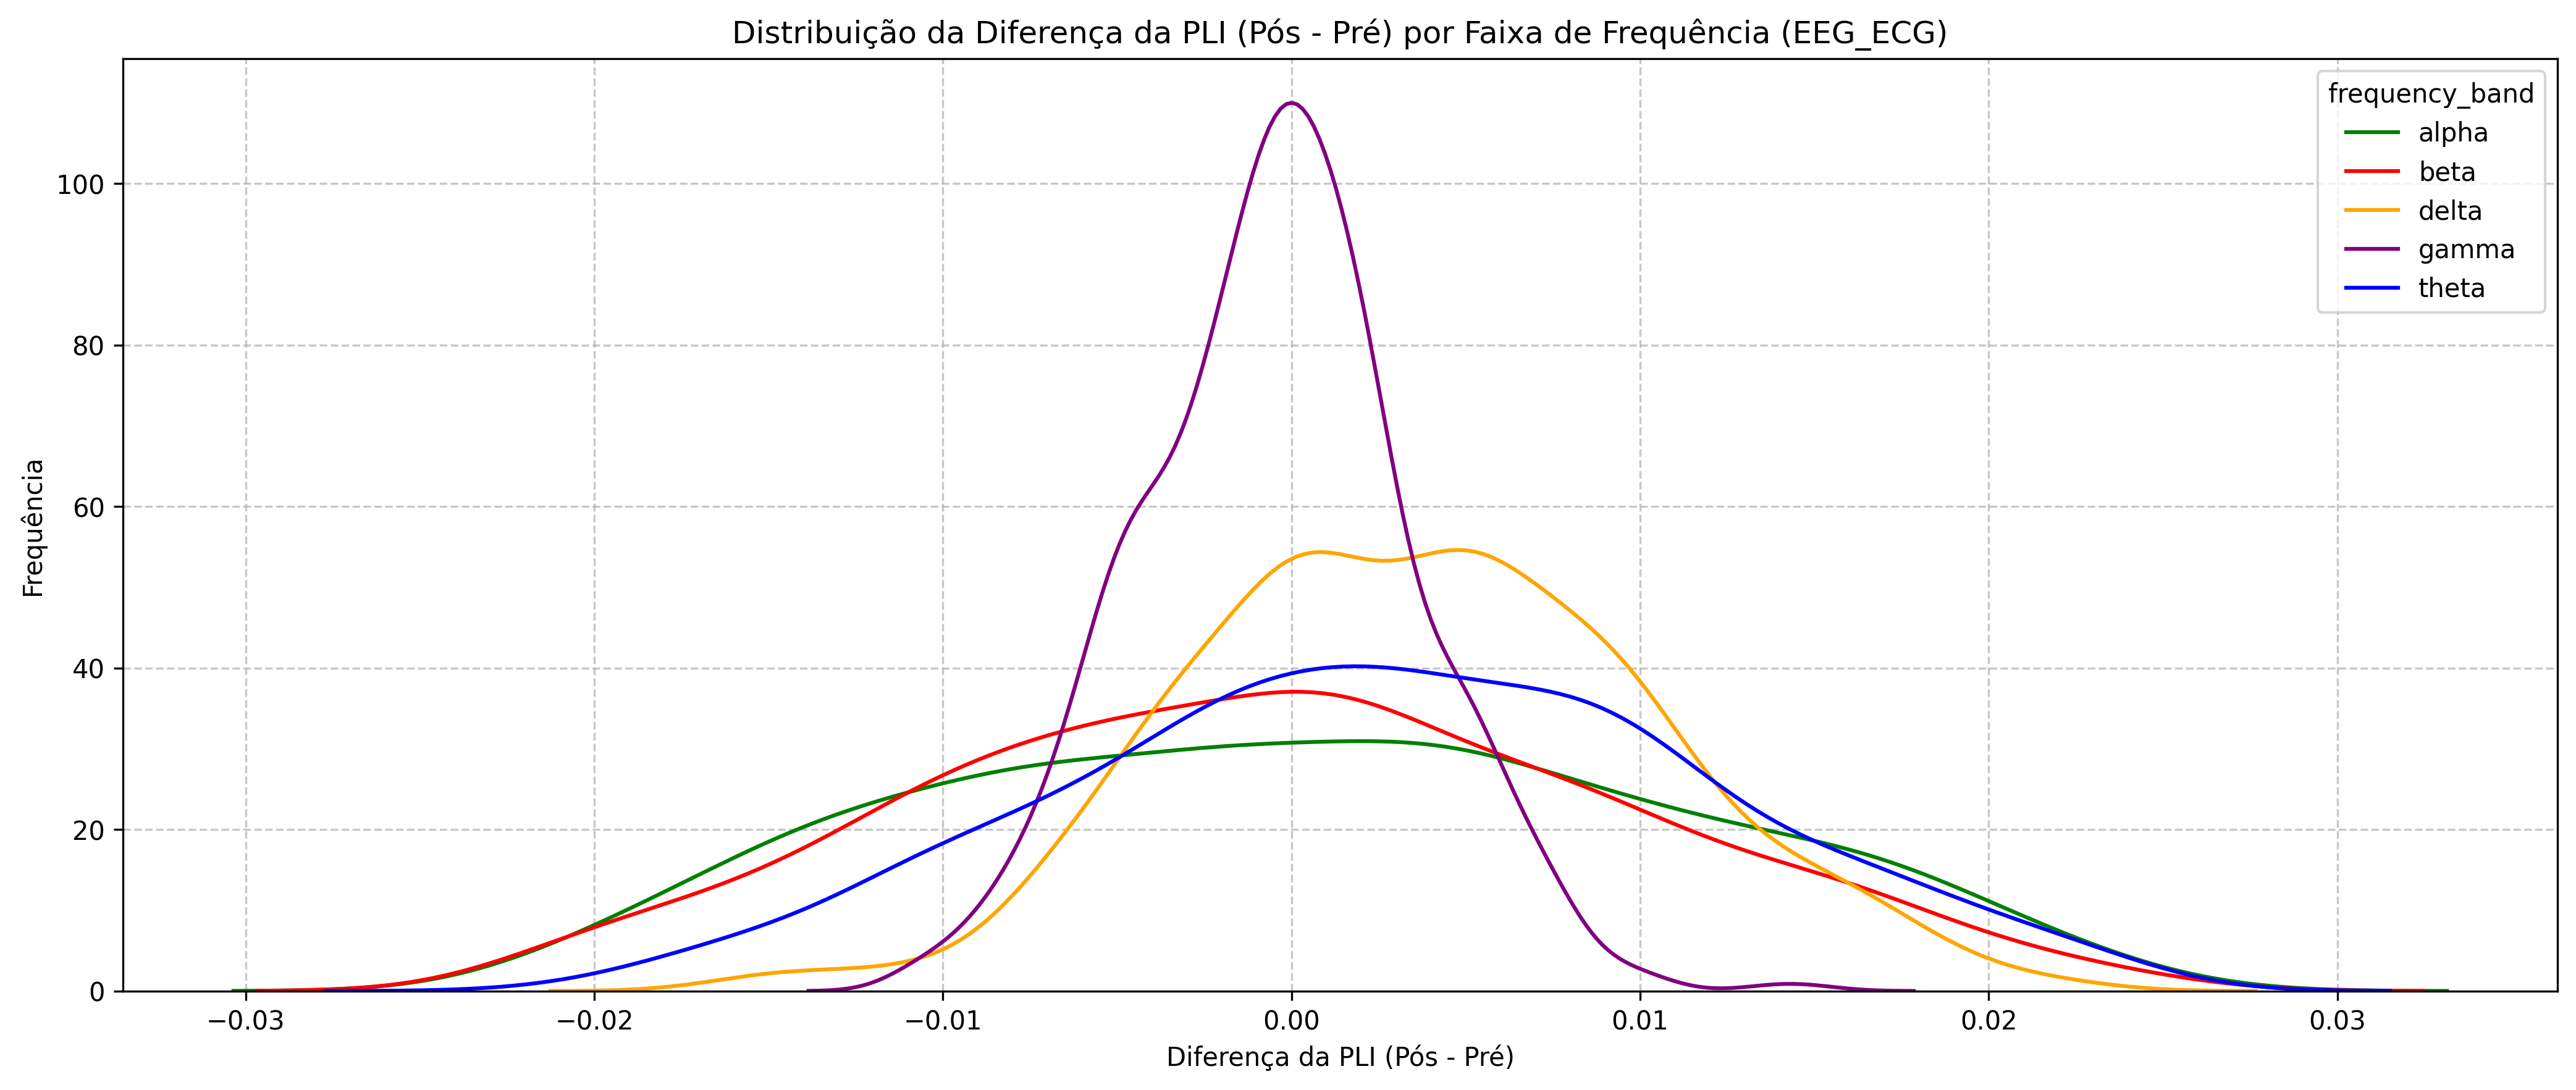
\includegraphics[width=0.8\textwidth]{figs/6_distribuicao_metricas_conectividade/Distribuição_da_Diferença_da_PLI_(Pós_-_Pré)_por_Faixa_de_Frequência_EEG_ECG.png}
    \caption{Distribuição da diferença da PLI (Pós -- Pré) por faixa de frequência para EEG-ECG.}
    \label{fig:pli_freq_eeg_ecg}
\end{figure}

\begin{figure}[htb]
    \centering
    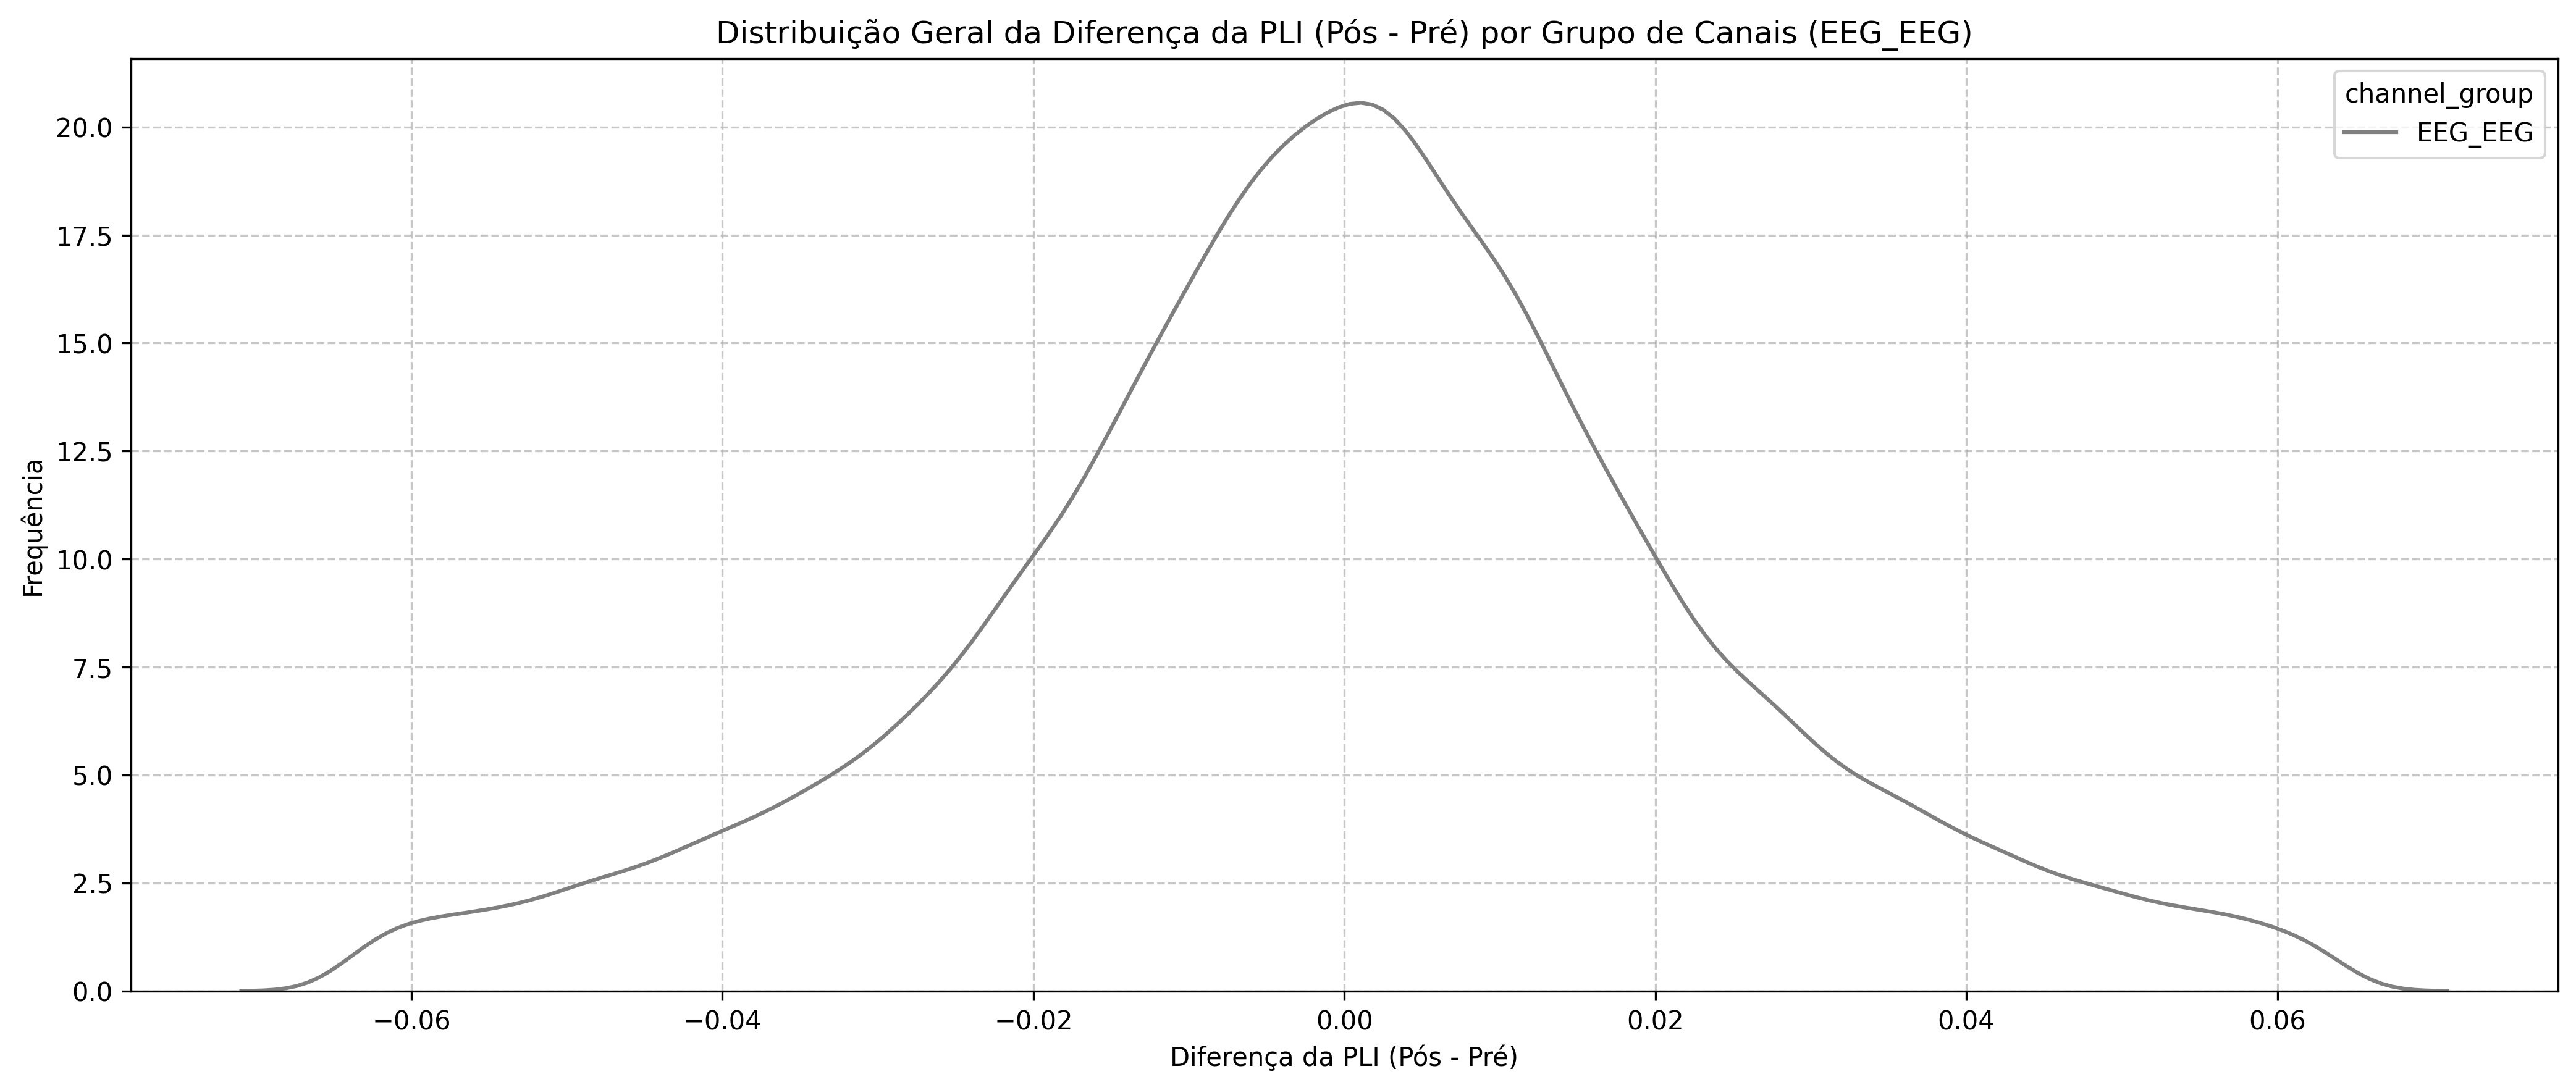
\includegraphics[width=0.8\textwidth]{figs/6_distribuicao_metricas_conectividade/Distribuição_Geral_da_Diferença_da_PLI_(Pós_-_Pré)_por_Grupo_de_Canais_EEG_EEG.png}
    \caption{Distribuição geral da diferença da PLI (Pós -- Pré) por grupo de canais (EEG-EEG).}
    \label{fig:pli_channel_eeg_eeg}
\end{figure}

\begin{figure}[htb]
    \centering
    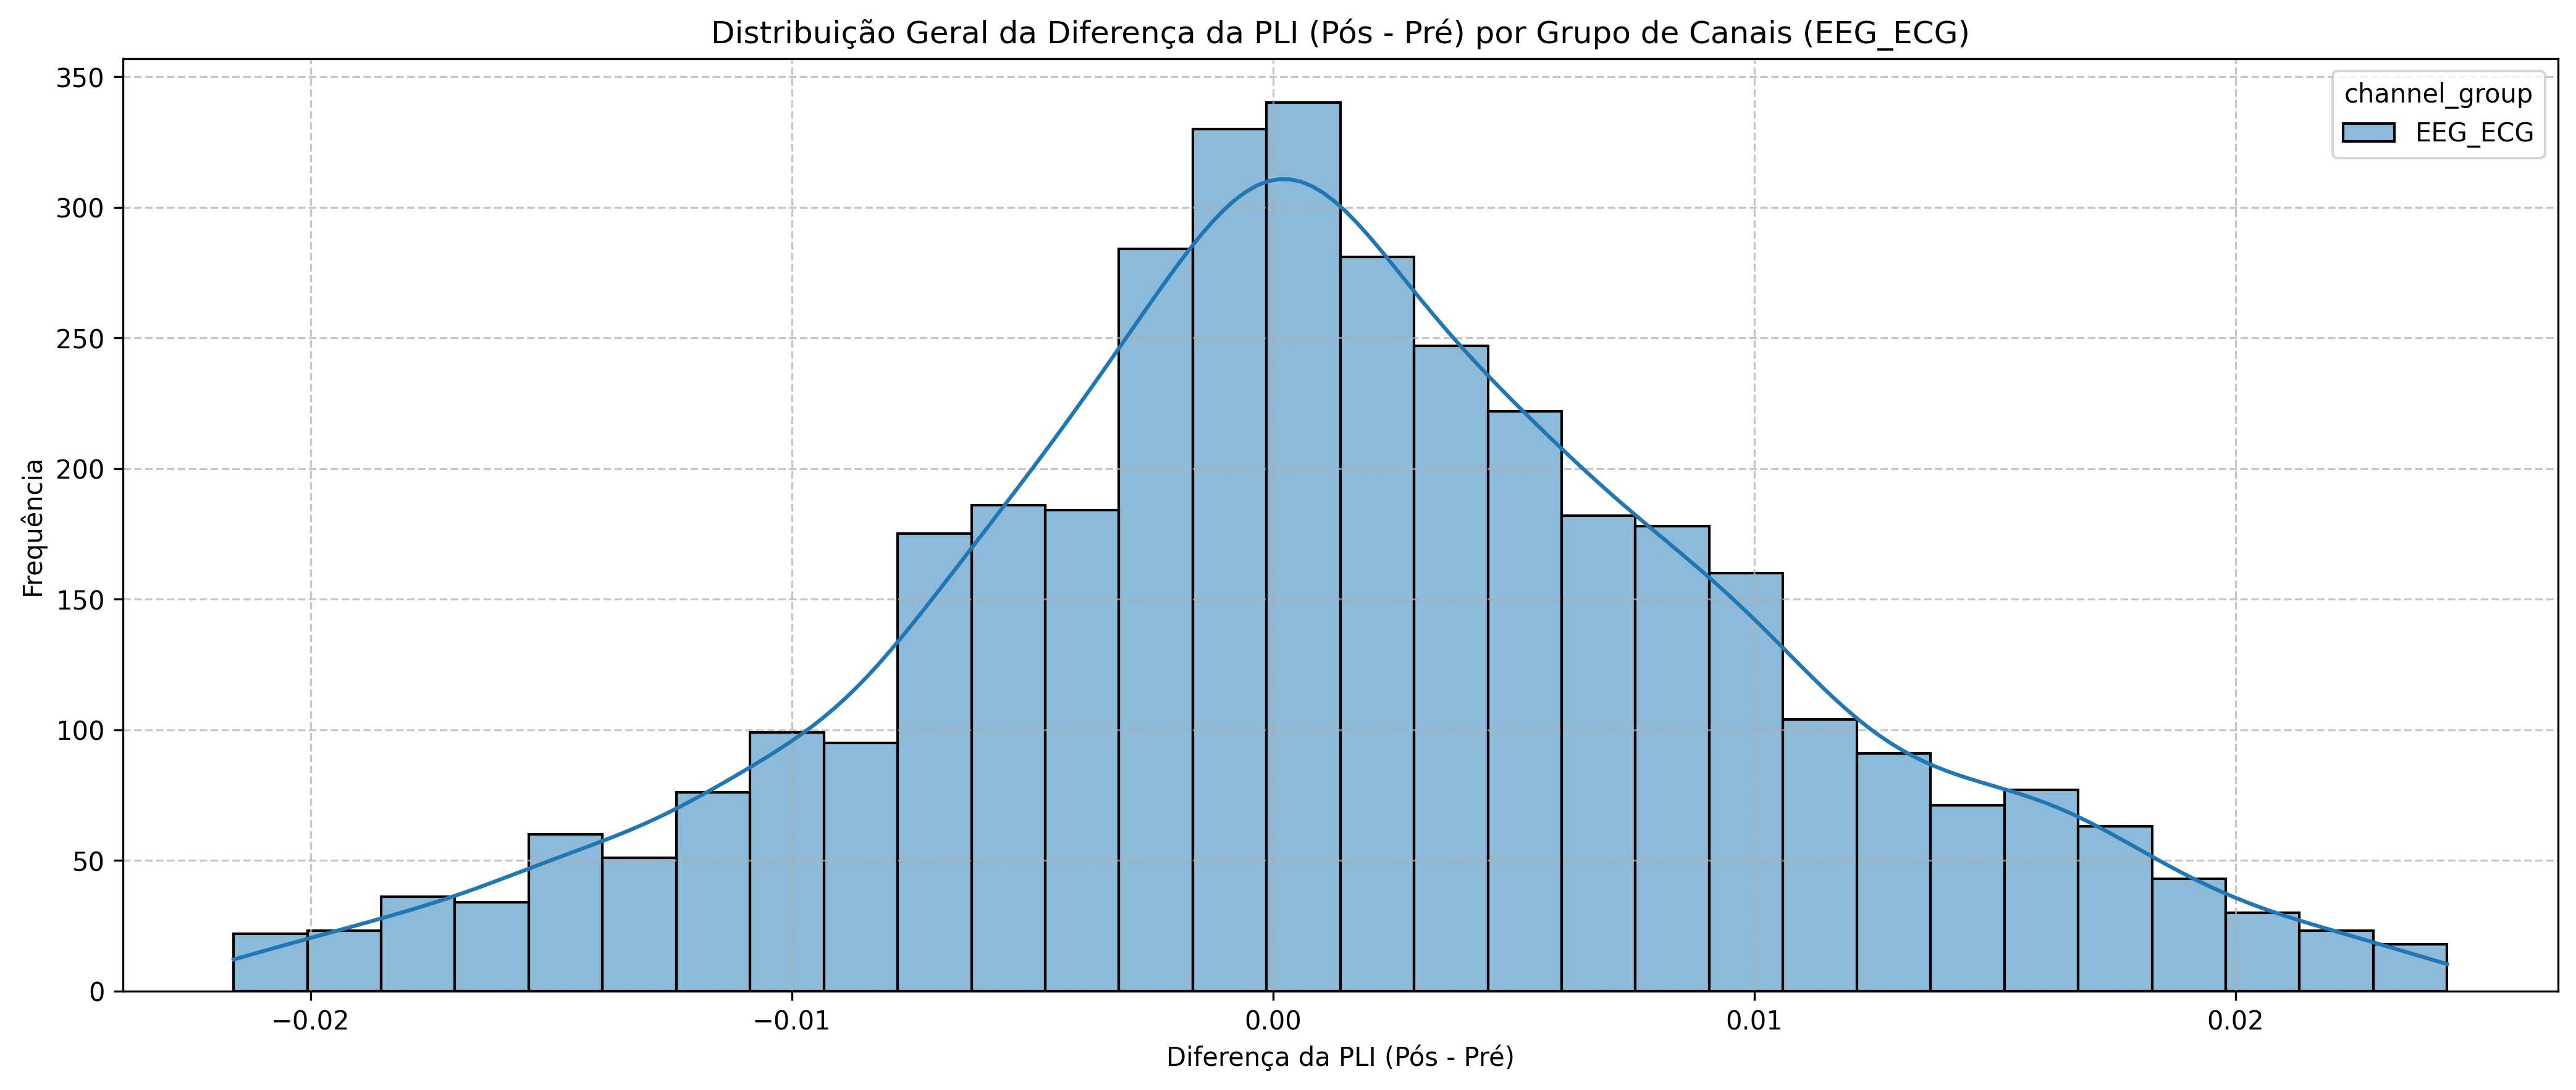
\includegraphics[width=0.8\textwidth]{figs/6_distribuicao_metricas_conectividade/Distribuição_Geral_da_Diferença_da_PLI_(Pós_-_Pré)_por_Grupo_de_Canais_EEG_ECG.png}
    \caption{Distribuição geral da diferença da PLI (Pós -- Pré) por grupo de canais (EEG-ECG).}
    \label{fig:pli_channel_eeg_ecg}
\end{figure}

\begin{figure}[htb]
    \centering
    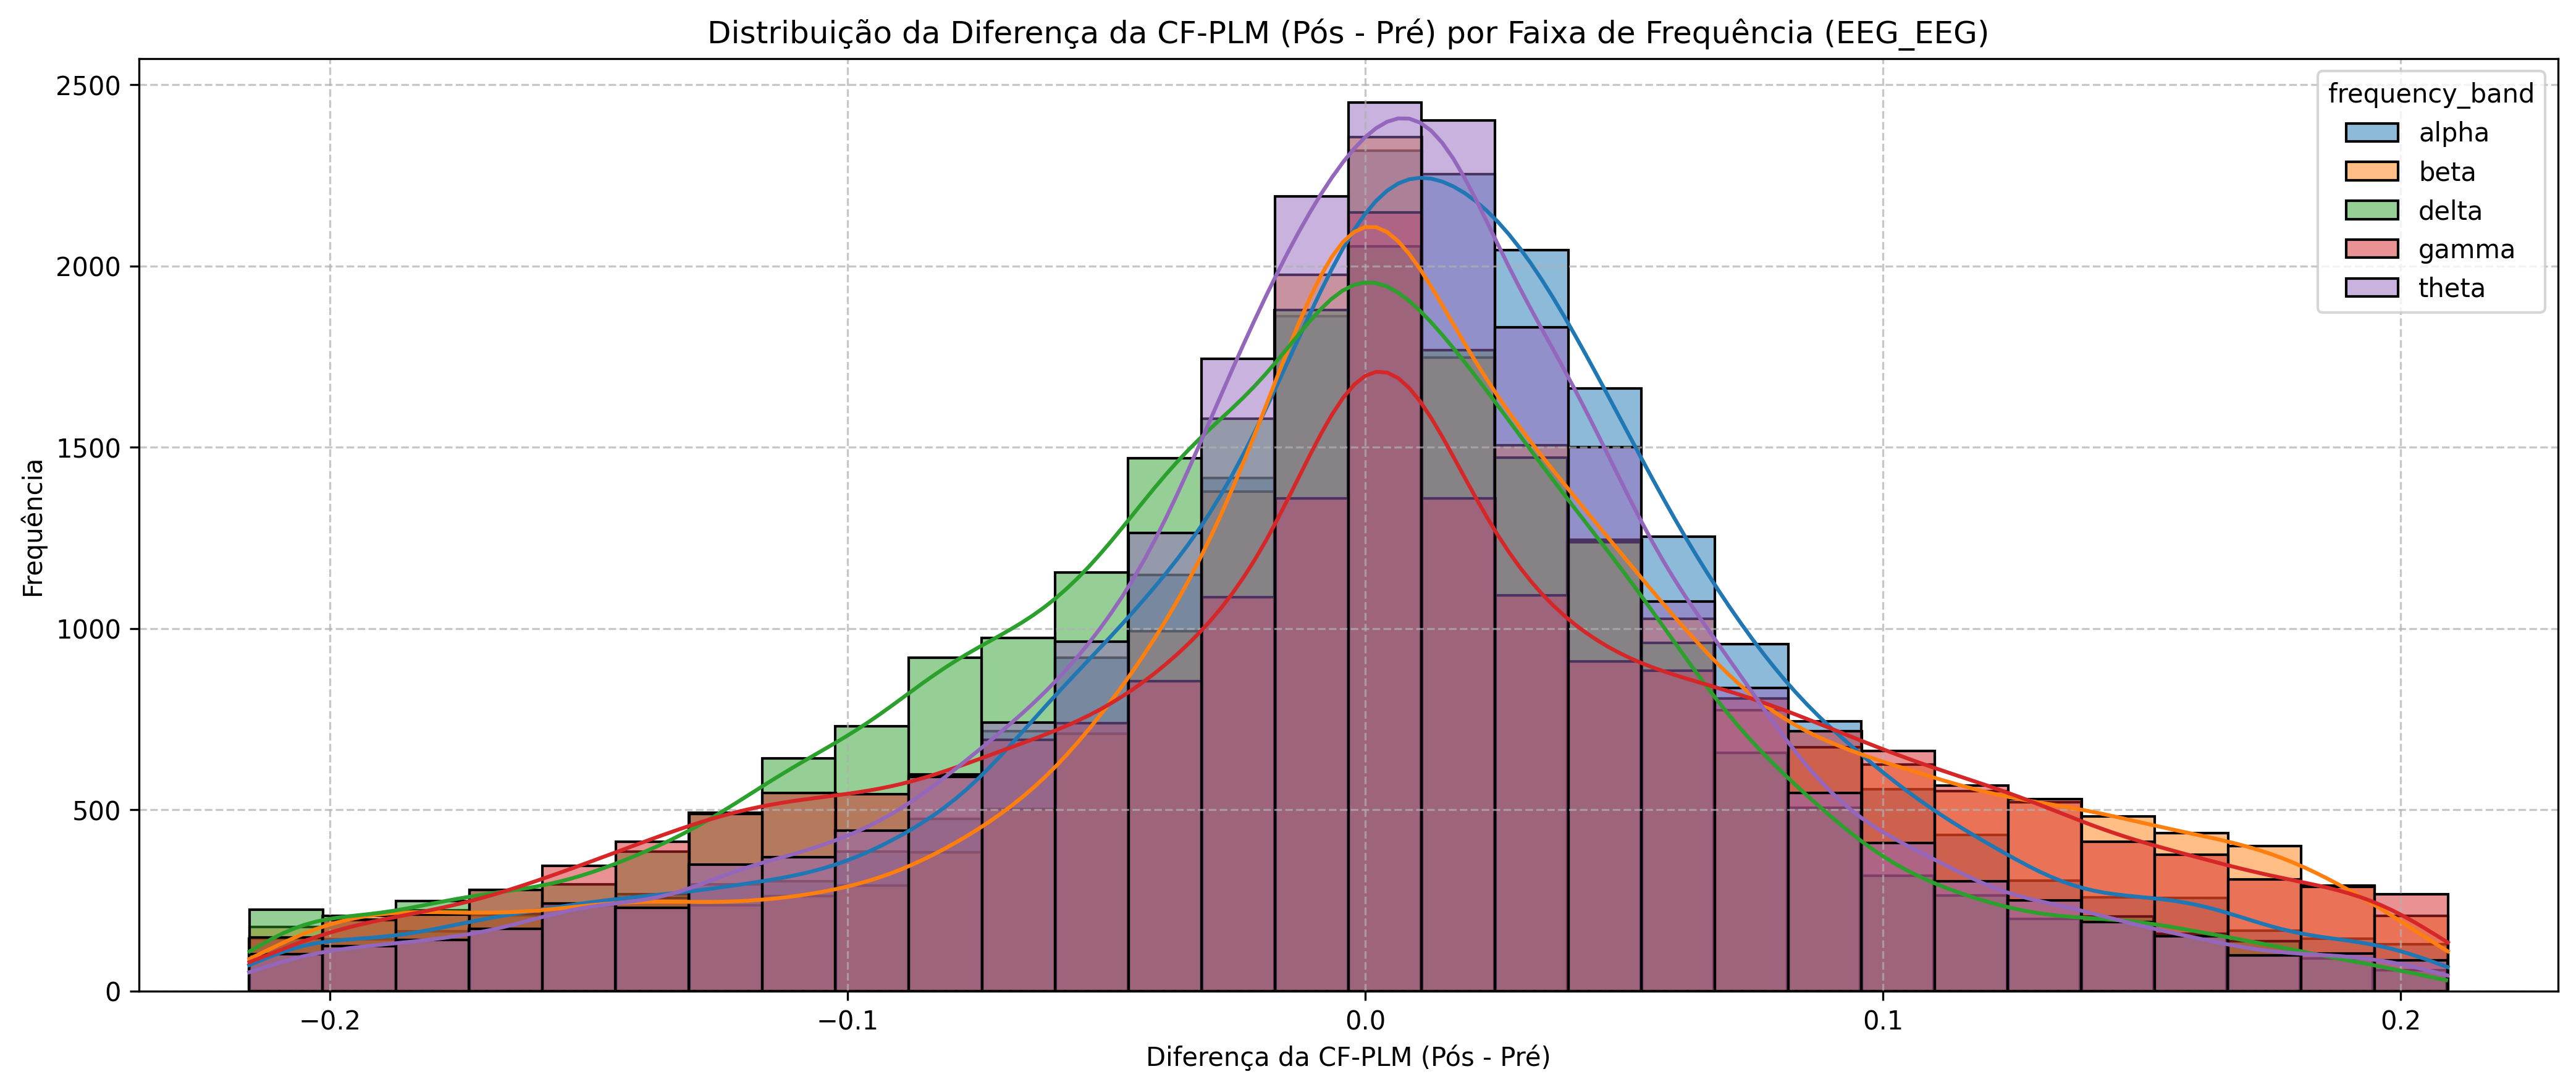
\includegraphics[width=0.8\textwidth]{figs/6_distribuicao_metricas_conectividade/Distribuição_da_Diferença_da_CF-PLM_(Pós_-_Pré)_por_Faixa_de_Frequência_EEG_EEG.png}
    \caption{Distribuição da diferença da CF-PLM (Pós -- Pré) por faixa de frequência para EEG-EEG.}
    \label{fig:cf_plm_freq_eeg_eeg}
\end{figure}

\begin{figure}[htb]
    \centering
    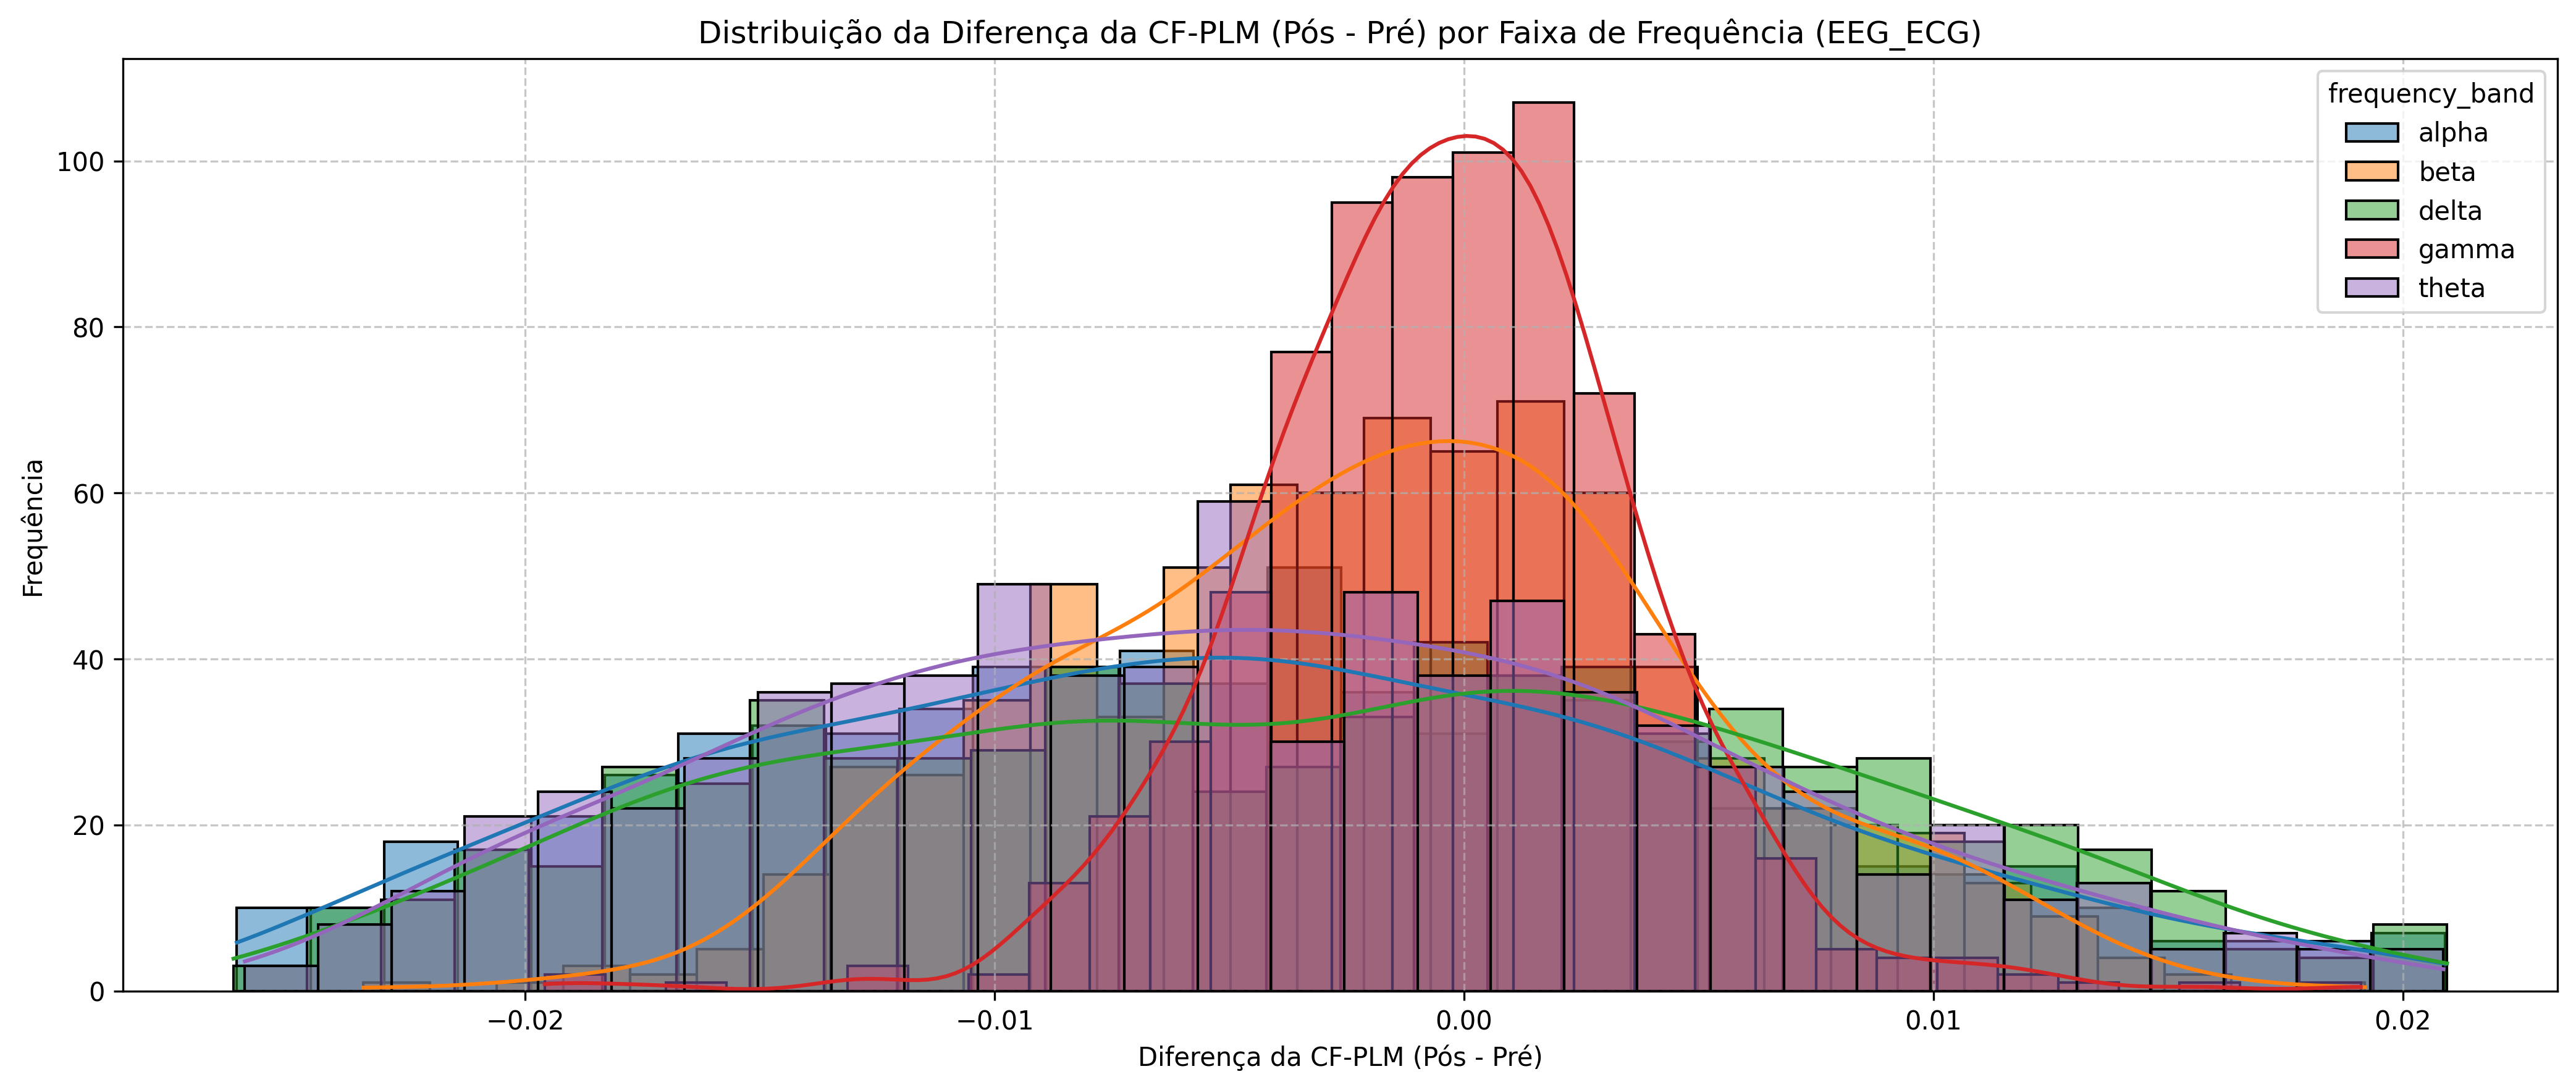
\includegraphics[width=0.8\textwidth]{figs/6_distribuicao_metricas_conectividade/Distribuição_da_Diferença_da_CF-PLM_(Pós_-_Pré)_por_Faixa_de_Frequência_EEG_ECG.png}
    \caption{Distribuição da diferença da CF-PLM (Pós -- Pré) por faixa de frequência para EEG-ECG.}
    \label{fig:cf_plm_freq_eeg_ecg}
\end{figure}

\begin{figure}[htb]
    \centering
    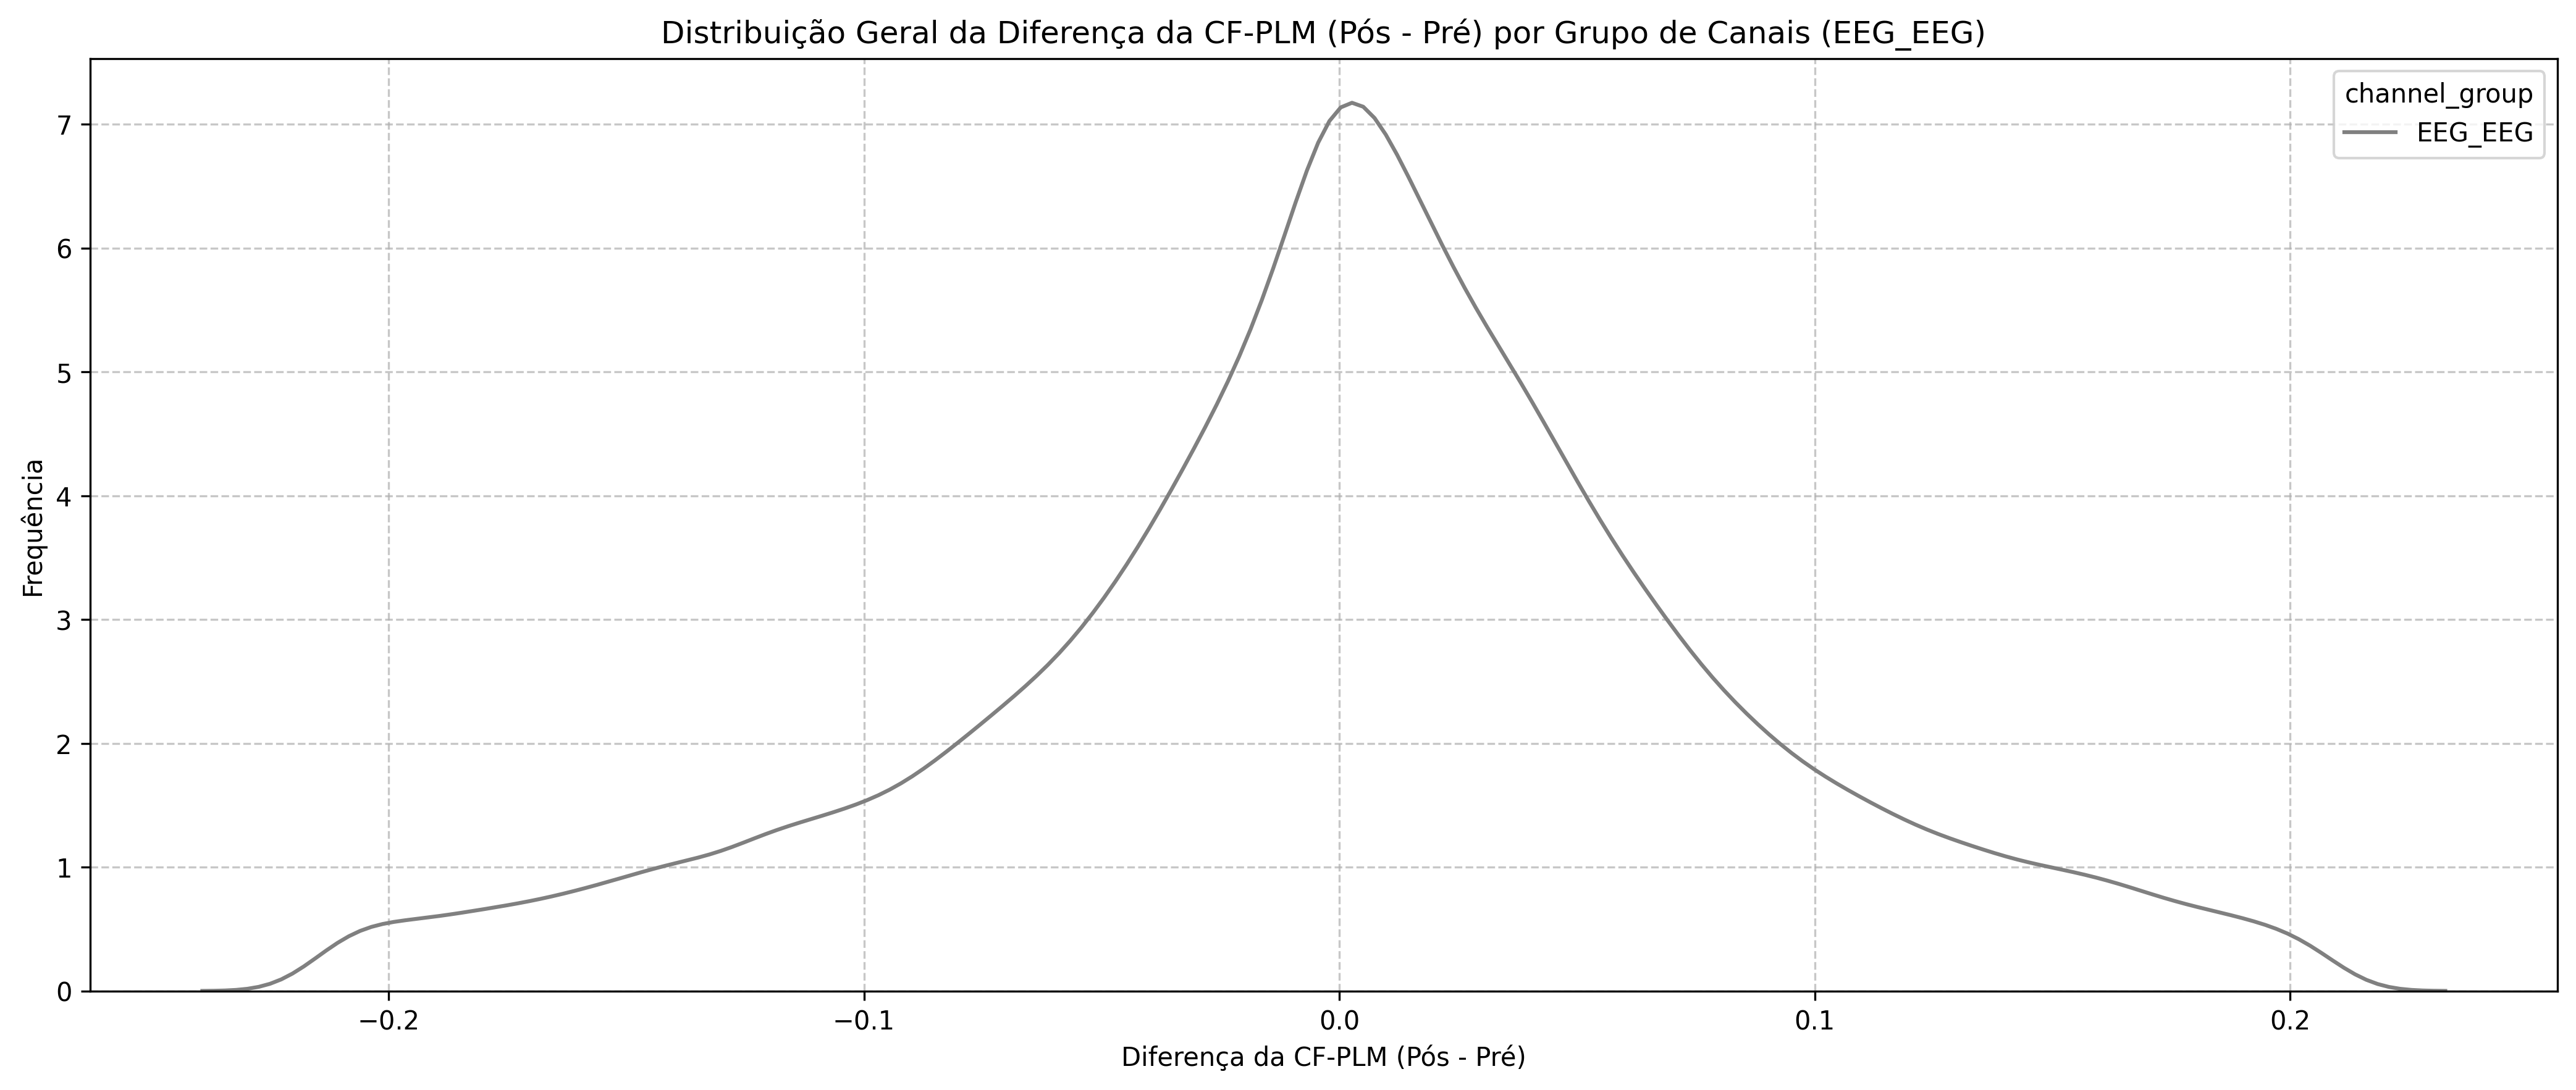
\includegraphics[width=0.8\textwidth]{figs/6_distribuicao_metricas_conectividade/Distribuição_Geral_da_Diferença_da_CF-PLM_(Pós_-_Pré)_por_Grupo_de_Canais_EEG_EEG.png}
    \caption{Distribuição geral da diferença da CF-PLM (Pós -- Pré) por grupo de canais (EEG-EEG).}
    \label{fig:cf_plm_channel_eeg_eeg}
\end{figure}

\begin{figure}[htb]
    \centering
    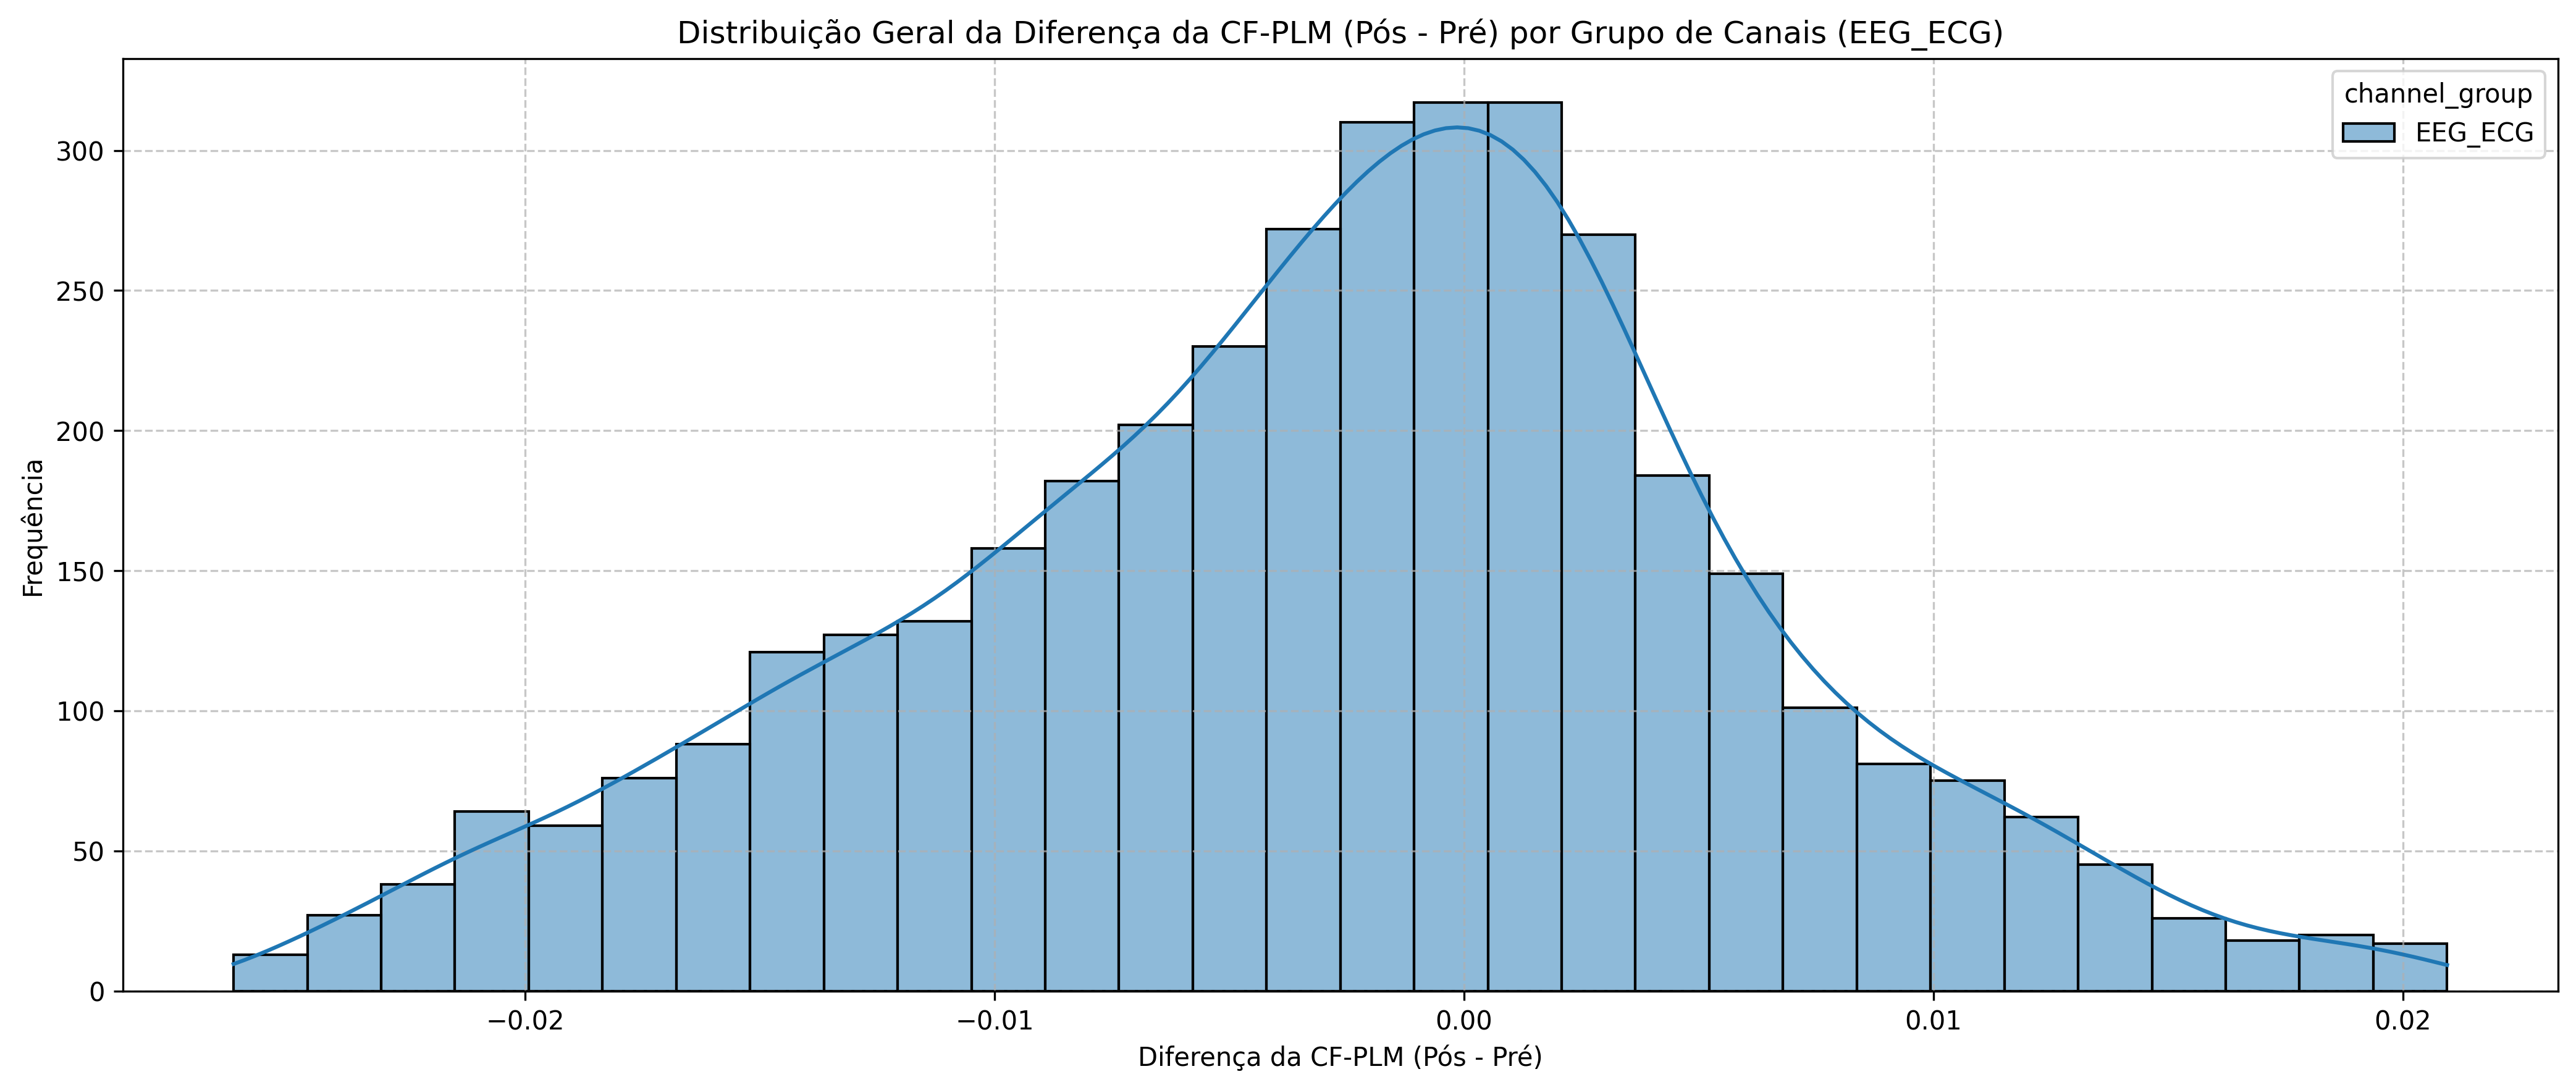
\includegraphics[width=0.8\textwidth]{figs/6_distribuicao_metricas_conectividade/Distribuição_Geral_da_Diferença_da_CF-PLM_(Pós_-_Pré)_por_Grupo_de_Canais_EEG_ECG.png}
    \caption{Distribuição geral da diferença da CF-PLM (Pós -- Pré) por grupo de canais (EEG-ECG).}
    \label{fig:cf_plm_channel_eeg_ecg}
\end{figure}

\subsubsection{Exemplo Individual por Métrica e Banda}
Para ilustrar de forma mais específica como essas distribuições se comportam em um caso individual, a Figura~\ref{fig:median_cf_plm_diff_ath4_alpha_eeg_ecg} exibe a distribuição da diferença da métrica \texttt{median\_cf\_plm\_diff} (Pós -- Pré) para o atleta 4, na banda \emph{alpha}, em pares EEG-ECG. Já a Figura~\ref{fig:median_pli_diff_ath4_alpha_eeg_eeg} apresenta a distribuição da diferença da \texttt{median\_pli\_diff} para o mesmo atleta 4 e banda alpha, porém em pares EEG-EEG.

\begin{figure}[htb]
    \centering
    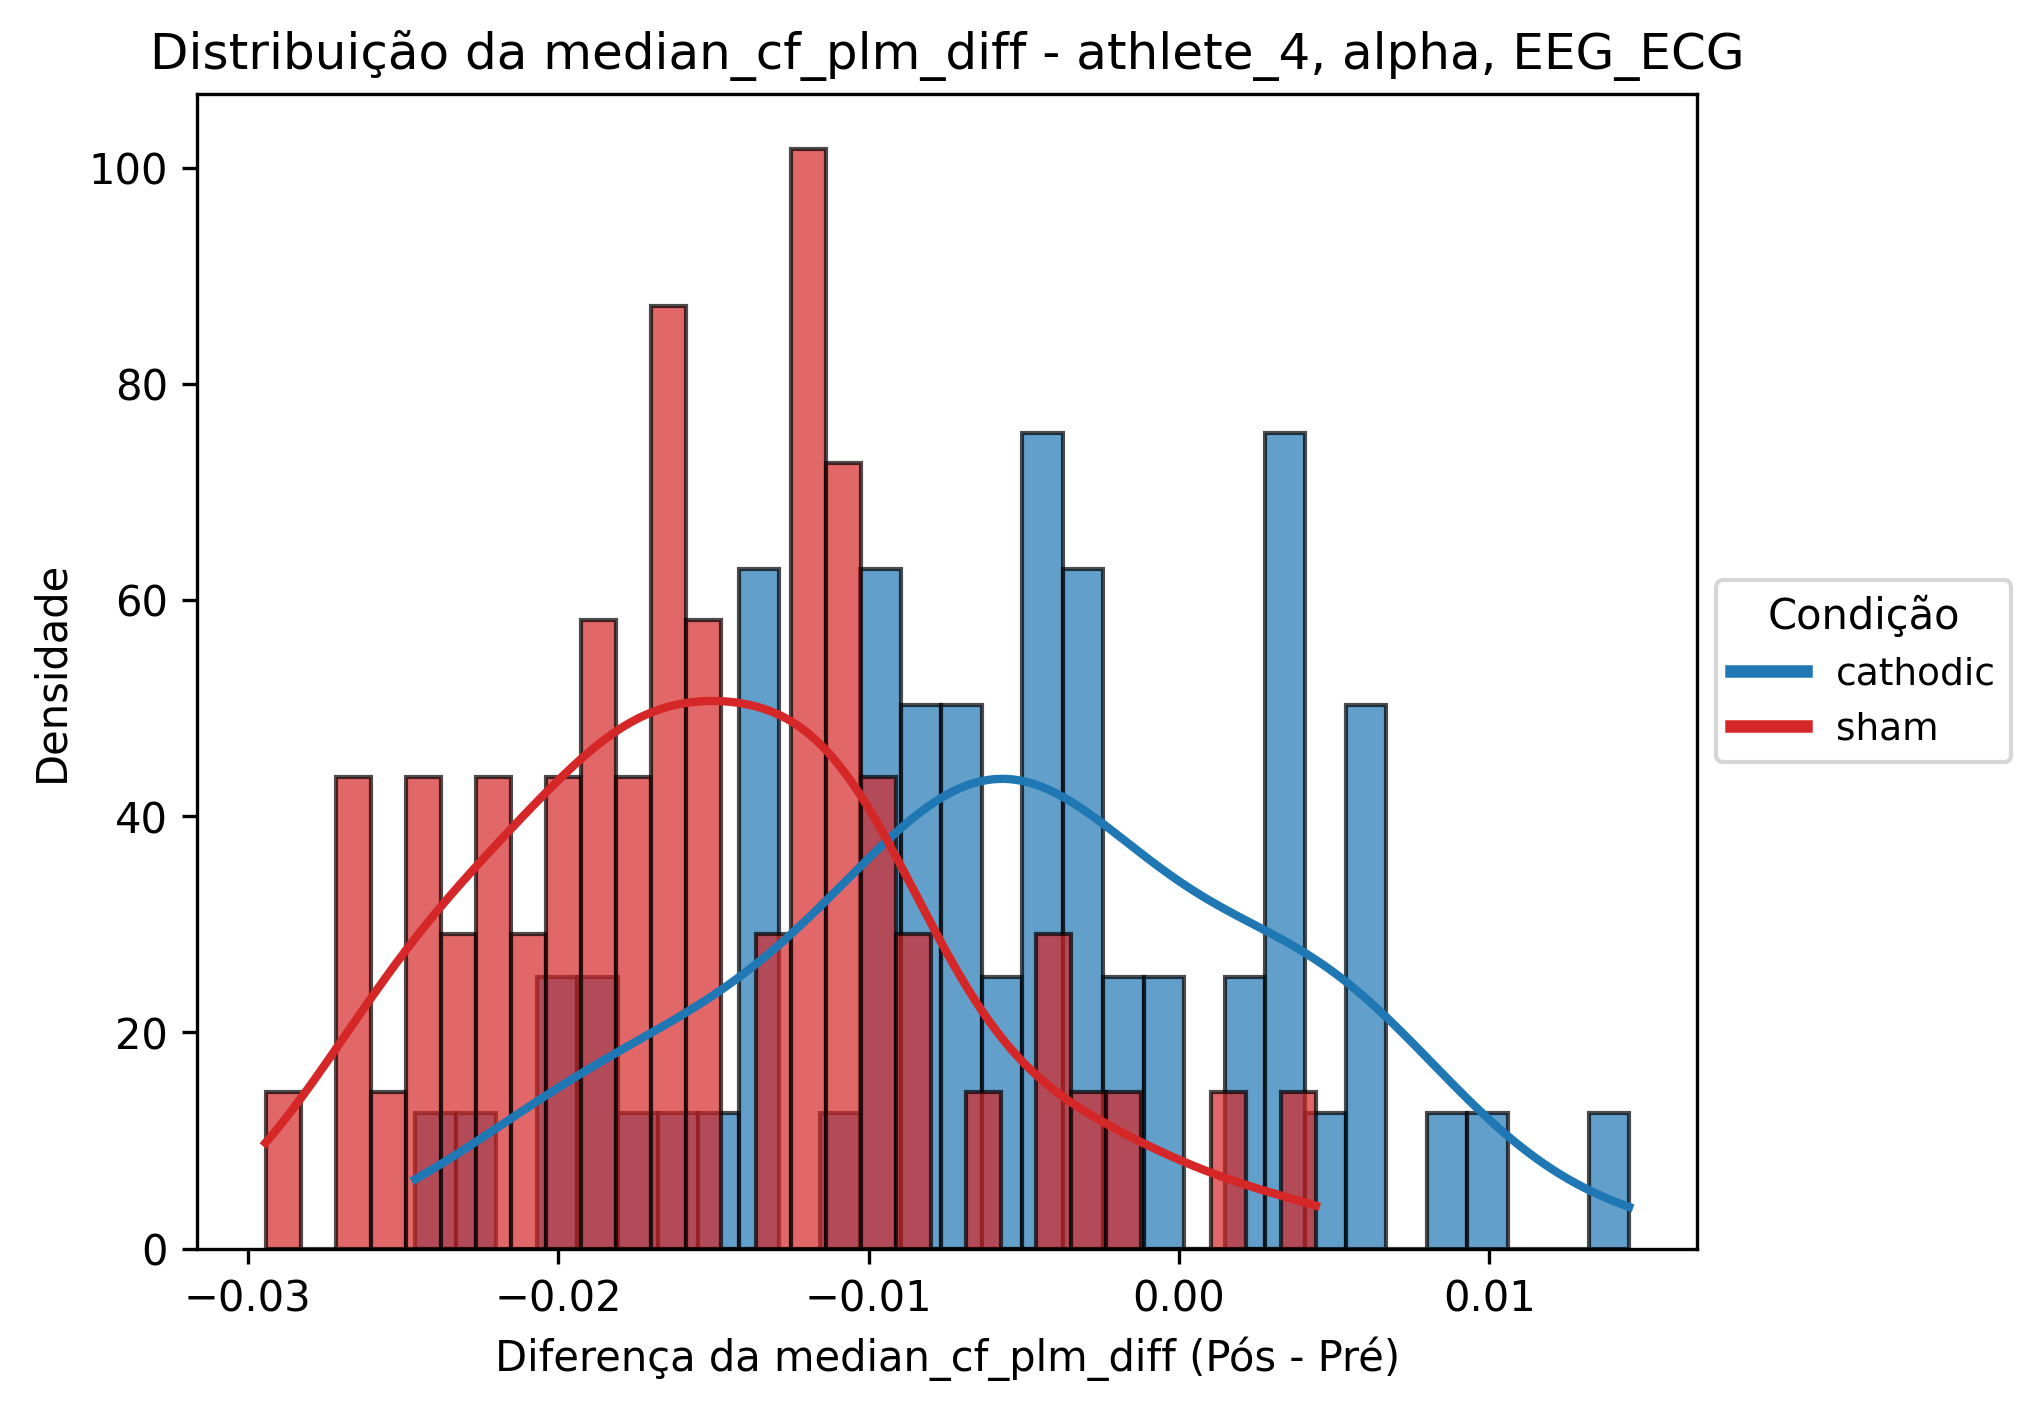
\includegraphics[width=0.8\textwidth]{figs/5_connectivity_metrics_individual_distribution/median_cf_plm_diff_athlete_4_alpha_EEG_ECG.png}
    \caption{Distribuição da \texttt{median\_cf\_plm\_diff} (Pós -- Pré) para o atleta 4, banda alpha, em pares EEG-ECG.}
    \label{fig:median_cf_plm_diff_ath4_alpha_eeg_ecg}
\end{figure}

\begin{figure}[htb]
    \centering
    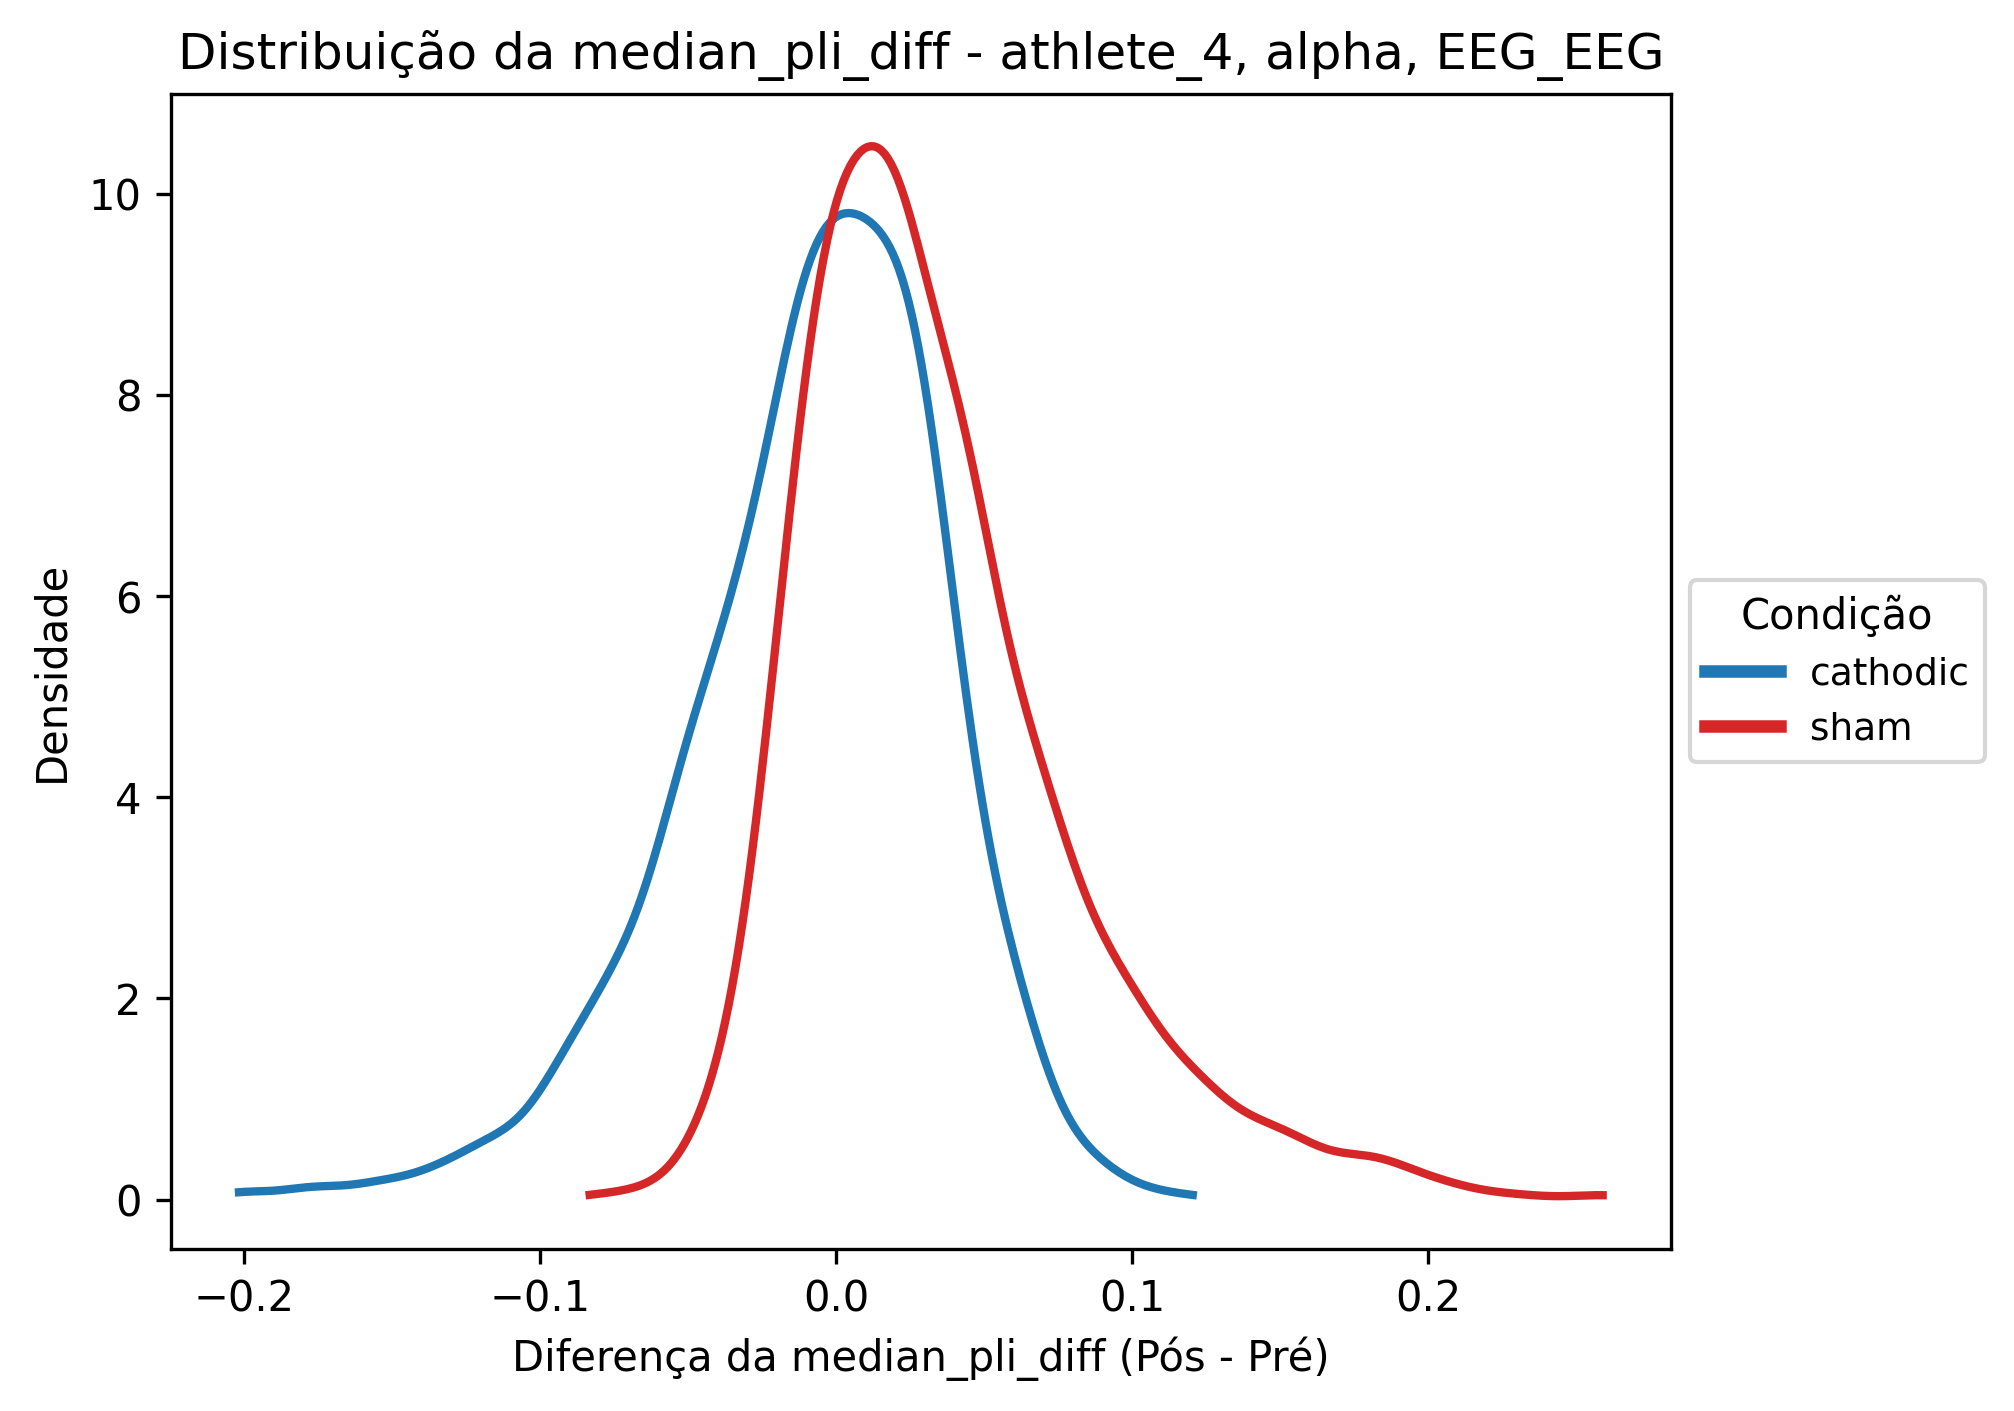
\includegraphics[width=0.8\textwidth]{figs/5_connectivity_metrics_individual_distribution/median_pli_diff_athlete_4_alpha_EEG_EEG.png}
    \caption{Distribuição da \texttt{median\_pli\_diff} (Pós -- Pré) para o atleta 4, banda alpha, em pares EEG-EEG.}
    \label{fig:median_pli_diff_ath4_alpha_eeg_eeg}
\end{figure}

Essas figuras exemplificam como as diferenças entre as condições \emph{cathodic} (azul) e \emph{sham} (vermelho) podem se sobrepor ou divergir. Em alguns casos, a curva KDE de uma condição pode deslocar-se à direita (indicando um aumento na métrica após a estimulação) ou à esquerda (indicando redução), enquanto em outros a sobreposição é substancial, sugerindo pouca mudança entre as condições. Esse tipo de análise individual é útil para verificar a variabilidade intra-sujeito e entender melhor se os efeitos observados são consistentes ou pontuais.

\section{Verificação de Normalidade e Escolha do Teste Estatístico}
Para definir se o teste estatístico a ser empregado é paramétrico ou não-paramétrico, é necessário verificar a normalidade das distribuições de interesse. Nesse contexto, testes como o de \emph{Shapiro-Wilk} ou \emph{Kolmogorov-Smirnov} podem ser aplicados para cada grupo de canais e faixa de frequência, tanto para a PLI quanto para a CF-PLM.

\paragraph{Considerações:}
\begin{itemize}
    \item \textbf{Tamanho amostral}: dada a quantidade relativamente grande de observações (após agregação), mesmo pequenas diferenças em relação à distribuição normal podem resultar em rejeição estatística da hipótese de normalidade.
    \item \textbf{Forma das distribuições}: visualmente, muitas distribuições parecem aproximadamente simétricas e unimodais. Ainda assim, pequenas assimetrias ou caudas mais alongadas podem exigir cautela na adoção de testes paramétricos.
    \item \textbf{Interpretação}: se a maioria das distribuições não satisfizer os critérios de normalidade (p.\,ex.\ p-valor $<$ 0.05), a análise inferencial subsequente pode se apoiar em testes não-paramétricos (por exemplo, \emph{Wilcoxon signed-rank} ou \emph{Mann-Whitney}).
\end{itemize}

\paragraph{Próximos Passos:}
\begin{itemize}
    \item Realizar os testes de normalidade (Shapiro-Wilk e/ou Kolmogorov-Smirnov) para cada combinação relevante de \emph{(faixa de frequência, grupo de canais)}.
    \item Avaliar as medidas de assimetria (\emph{skewness}) e curtose (\emph{kurtosis}) para confirmar a adequação de testes paramétricos ou justificar o uso de métodos não-paramétricos.
\end{itemize}

Com base nessa análise preliminar, será possível conduzir as etapas seguintes de inferência estatística, considerando as particularidades de cada métrica (PLI e CF-PLM) e garantindo uma avaliação mais robusta das diferenças entre condições.

\section{Testes de Normalidade e Decisão sobre o Tipo de Teste Estatístico}
A escolha entre testes paramétricos e não paramétricos depende fundamentalmente da distribuição dos dados. Para as métricas de conectividade (median\_plv\_diff, median\_pli\_diff e median\_cf\_plm\_diff) agrupadas nos grupos \texttt{EEG\_EEG} e \texttt{EEG\_ECG}, aplicamos uma série de testes de normalidade, a saber: Shapiro-Wilk, Kolmogorov-Smirnov, Anderson-Darling, D'Agostino's K-squared, Jarque-Bera e Lilliefors. Além disso, para atenuar o efeito de valores extremos, os testes foram realizados tanto com os dados originais quanto após a remoção de outliers utilizando o método do \emph{Interquartile Range} (IQR).

\paragraph{Motivações e Procedimentos:}
\begin{itemize}
    \item \textbf{Objetivo:} Verificar se as distribuições das diferenças (Pós -- Pré) seguem uma forma aproximadamente gaussiana, o que permitiria o uso de testes paramétricos.
    \item \textbf{Procedimento:} 
    \begin{itemize}
        \item Os dados foram agrupados por \texttt{channel\_group} (EEG\_EEG e EEG\_ECG) e para cada métrica.
        \item Foram aplicados os testes de normalidade com e sem outliers, permitindo avaliar o efeito destes na distribuição.
    \end{itemize}
\end{itemize}

\paragraph{Principais Resultados:}
\begin{itemize}
    \item \textbf{Grupo EEG\_EEG:}
    \begin{itemize}
        \item Para \texttt{median\_plv\_diff}, todos os testes (Shapiro-Wilk, Kolmogorov-Smirnov, Anderson-Darling, D'Agostino, Jarque-Bera e Lilliefors) apresentaram p-valores inferiores a 0,001, rejeitando a hipótese de normalidade, mesmo após a remoção de aproximadamente 9,44\% dos dados como outliers.
        \item Similarmente, para \texttt{median\_pli\_diff} e \texttt{median\_cf\_plm\_diff}, os testes indicaram desvios significativos da normalidade (p-valores muito baixos), mesmo após a filtragem de outliers (10,66\% e 10,65\% dos dados, respectivamente).
    \end{itemize}
    \item \textbf{Grupo EEG\_ECG:}
    \begin{itemize}
        \item Embora a remoção de outliers tenha melhorado levemente a distribuição de \texttt{median\_plv\_diff} (com alguns testes chegando a p-valores marginalmente aceitáveis), para \texttt{median\_pli\_diff} e \texttt{median\_cf\_plm\_diff} os testes continuaram a rejeitar a normalidade (p-valores próximos de zero na maioria dos casos).
    \end{itemize}
\end{itemize}

\paragraph{Interpretação e Decisão Metodológica:}  
Os resultados dos testes de normalidade demonstram que, em sua maioria, as distribuições das diferenças nas métricas de conectividade não se comportam de maneira normal, mesmo após a remoção de outliers. Essa violação do pressuposto de normalidade indica que a aplicação de testes paramétricos (que assumem uma distribuição gaussiana dos dados) poderia levar a inferências incorretas. Portanto, optamos por utilizar testes não paramétricos para as análises estatísticas subsequentes, garantindo robustez e validade às conclusões sem a necessidade de assumir normalidade dos dados.
